% ####################################################################
% Basic configuration of Beamera class and Jagiellonian theme
% ####################################################################
\RequirePackage[l2tabu, orthodox]{nag}



\ifx\PresentationStyle\notset
  \def\PresentationStyle{dark}
\fi



% Options: t - align frame text to the top.
\documentclass[10pt,t]{beamer}
\mode<presentation>
\usetheme[style=\PresentationStyle]{jagiellonian}




% ------------------------------------------------------------------------------------
% Procesing configuration files of Jagiellonian theme located
% in the directory "preambule"
% ------------------------------------------------------------------------------------
% Configuration for polish language
% Need description
\usepackage[polish]{babel}
% Need description
\usepackage[MeX]{polski}



% ------------------------------
% Better support of polish chars in technical parts of PDF
% ------------------------------
\hypersetup{pdfencoding=auto,psdextra}

% Package "textpos" give as enviroment "textblock" which is very usefull in
% arranging text on slides.

% This is standard configuration of "textpos"
\usepackage[overlay,absolute]{textpos}

% If you need to see bounds of "textblock's" comment line above and uncomment
% one below.

% Caution! When showboxes option is on significant ammunt of space is add
% to the top of textblock and as such, everyting put in them gone down.
% We need to check how to remove this bug.

% \usepackage[showboxes,overlay,absolute]{textpos}



% Setting scale length for package "textpos"
\setlength{\TPHorizModule}{10mm}
\setlength{\TPVertModule}{\TPHorizModule}


% ---------------------------------------
% Packages written for lectures "Geometria 3D dla twórców gier wideo"
% ---------------------------------------
% \usepackage{./Geometry3DPackages/Geometry3D}
% \usepackage{./Geometry3DPackages/Geometry3DIndices}
% \usepackage{./Geometry3DPackages/Geometry3DTikZStyle}
% \usepackage{./ProgramowanieSymulacjiFizykiPaczki/ProgramowanieSymulacjiFizykiTikZStyle}
% \usepackage{./Geometry3DPackages/mathcommands}


% ---------------------------------------
% Importing TikZ's libraries
% ---------------------------------------
\usetikzlibrary{arrows.meta}
\usetikzlibrary{positioning}





% % Configuration package "bm" that need for making bold symbols
\newcommand{\bmmax}{0}
\newcommand{\hmmax}{0}
\usepackage{bm}




% ---------------------------------------
% Packages for scientific texts
% ---------------------------------------
% \let\lll\undefined  % Sometimes you must use this line to allow
% "amsmath" package to works with packages with packages for polish
% languge imported
% /preambul/LanguageSettings/JagiellonianPolishLanguageSettings.tex.
% This comments (probably) removes polish letter Ł.
\usepackage{amsmath}  % Packages from American Mathematical Society (AMS)
\usepackage{amssymb}
\usepackage{amscd}
\usepackage{amsthm}
\usepackage{siunitx}  % Package for typsetting SI units.
\usepackage{upgreek}  % Better looking greek letters.
% Example of using upgreek: pi = \uppi


\usepackage{calrsfs}  % Zmienia czcionkę kaligraficzną w \mathcal
% na ładniejszą. Może w innych miejscach robi to samo, ale o tym nic
% nie wiem.







% !!!!!!!!!!!!!!!!!!!!!!!!!!!!!!
% !!!!!!!!!!!!!!!!!!!!!!!!!!!!!!
% EVIL STUFF
\if\JUlogotitle1
\edef\LogoJUPath{LogoJU_\JUlogoLang/LogoJU_\JUlogoShape_\JUlogoColor.pdf}
\titlegraphic{\hfill\includegraphics[scale=0.22]
{./JagiellonianPictures/\LogoJUPath}}
\fi

% ---------------------------------------
% Commands for handling colors
% ---------------------------------------


% Command for setting normal text color for some text in math modestyle
% Text color depend on used style of Jagiellonian

% Beamer version of command
\newcommand{\TextWithNormalTextColor}[1]{%
  {\color{jNormalTextFGColor}
    \setbeamercolor{math text}{fg=jNormalTextFGColor} {#1}}
}

% Article and similar classes version of command
% \newcommand{\TextWithNormalTextColor}[1]{%
%   {\color{jNormalTextsFGColor} {#1}}
% }



% Beamer version of command
\newcommand{\NormalTextInMathMode}[1]{%
  {\color{jNormalTextFGColor}
    \setbeamercolor{math text}{fg=jNormalTextFGColor} \text{#1}}
}


% Article and similar classes version of command
% \newcommand{\NormalTextInMathMode}[1]{%
%   {\color{jNormalTextsFGColor} \text{#1}}
% }




% Command that sets color of some mathematical text to the same color
% that has normal text in header (?)

% Beamer version of the command
\newcommand{\MathTextFrametitleFGColor}[1]{%
  {\color{jFrametitleFGColor}
    \setbeamercolor{math text}{fg=jFrametitleFGColor} #1}
}

% Article and similar classes version of the command
% \newcommand{\MathTextWhiteColor}[1]{{\color{jFrametitleFGColor} #1}}





% Command for setting color of alert text for some text in math modestyle

% Beamer version of the command
\newcommand{\MathTextAlertColor}[1]{%
  {\color{jOrange} \setbeamercolor{math text}{fg=jOrange} #1}
}

% Article and similar classes version of the command
% \newcommand{\MathTextAlertColor}[1]{{\color{jOrange} #1}}





% Command that allow you to sets chosen color as the color of some text into
% math mode. Due to some nuances in the way that Beamer handle colors
% it not work in all cases. We hope that in the future we will improve it.

% Beamer version of the command
\newcommand{\SetMathTextColor}[2]{%
  {\color{#1} \setbeamercolor{math text}{fg=#1} #2}
}


% Article and similar classes version of the command
% \newcommand{\SetMathTextColor}[2]{{\color{#1} #2}}










% ---------------------------------------
% Commands for few special slides
% ---------------------------------------
\newcommand{\EndingSlide}[1]{%
  \begin{frame}[standout]

    \begingroup

    \color{jFrametitleFGColor}

    #1

    \endgroup

  \end{frame}
}










% ---------------------------------------
% Commands for setting background pictures for some slides
% ---------------------------------------
\newcommand{\TitleBackgroundPicture}
{./JagiellonianPictures/Backgrounds/LajkonikDark.png}
\newcommand{\SectionBackgroundPicture}
{./JagiellonianPictures/Backgrounds/LajkonikLight.png}



\newcommand{\TitleSlideWithPicture}{%
  \begingroup

  \usebackgroundtemplate{%
    \includegraphics[height=\paperheight]{\TitleBackgroundPicture}}

  \maketitle

  \endgroup
}





\newcommand{\SectionSlideWithPicture}[1]{%
  \begingroup

  \usebackgroundtemplate{%
    \includegraphics[height=\paperheight]{\SectionBackgroundPicture}}

  \setbeamercolor{titlelike}{fg=normal text.fg}

  \section{#1}

  \endgroup
}










% ---------------------------------------
% Commands for lectures "Geometria 3D dla twórców gier wideo"
% Polish version
% ---------------------------------------
% Komendy teraz wykomentowane były potrzebne, gdy loga były na niebieskim
% tle, nie na białym. A są na białym bo tego chcieli w biurze projektu.
% \newcommand{\FundingLogoWhitePicturePL}
% {./PresentationPictures/CommonPictures/logotypFundusze_biale_bez_tla2.pdf}
\newcommand{\FundingLogoColorPicturePL}
{./PresentationPictures/CommonPictures/European_Funds_color_PL.pdf}
% \newcommand{\EULogoWhitePicturePL}
% {./PresentationPictures/CommonPictures/logotypUE_biale_bez_tla2.pdf}
\newcommand{\EUSocialFundLogoColorPicturePL}
{./PresentationPictures/CommonPictures/EU_Social_Fund_color_PL.pdf}
% \newcommand{\ZintegrUJLogoWhitePicturePL}
% {./PresentationPictures/CommonPictures/zintegruj-logo-white.pdf}
\newcommand{\ZintegrUJLogoColorPicturePL}
{./PresentationPictures/CommonPictures/ZintegrUJ_color.pdf}
\newcommand{\JULogoColorPicturePL}
{./JagiellonianPictures/LogoJU_PL/LogoJU_A_color.pdf}





\newcommand{\GeometryThreeDSpecialBeginningSlidePL}{%
  \begin{frame}[standout]

    \begin{textblock}{11}(1,0.7)

      \begin{flushleft}

        \mdseries

        \footnotesize

        \color{jFrametitleFGColor}

        Materiał powstał w ramach projektu współfinansowanego ze środków
        Unii Europejskiej w ramach Europejskiego Funduszu Społecznego
        POWR.03.05.00-00-Z309/17-00.

      \end{flushleft}

    \end{textblock}





    \begin{textblock}{10}(0,2.2)

      \tikz \fill[color=jBackgroundStyleLight] (0,0) rectangle (12.8,-1.5);

    \end{textblock}


    \begin{textblock}{3.2}(1,2.45)

      \includegraphics[scale=0.3]{\FundingLogoColorPicturePL}

    \end{textblock}


    \begin{textblock}{2.5}(3.7,2.5)

      \includegraphics[scale=0.2]{\JULogoColorPicturePL}

    \end{textblock}


    \begin{textblock}{2.5}(6,2.4)

      \includegraphics[scale=0.1]{\ZintegrUJLogoColorPicturePL}

    \end{textblock}


    \begin{textblock}{4.2}(8.4,2.6)

      \includegraphics[scale=0.3]{\EUSocialFundLogoColorPicturePL}

    \end{textblock}

  \end{frame}
}



\newcommand{\GeometryThreeDTwoSpecialBeginningSlidesPL}{%
  \begin{frame}[standout]

    \begin{textblock}{11}(1,0.7)

      \begin{flushleft}

        \mdseries

        \footnotesize

        \color{jFrametitleFGColor}

        Materiał powstał w ramach projektu współfinansowanego ze środków
        Unii Europejskiej w ramach Europejskiego Funduszu Społecznego
        POWR.03.05.00-00-Z309/17-00.

      \end{flushleft}

    \end{textblock}





    \begin{textblock}{10}(0,2.2)

      \tikz \fill[color=jBackgroundStyleLight] (0,0) rectangle (12.8,-1.5);

    \end{textblock}


    \begin{textblock}{3.2}(1,2.45)

      \includegraphics[scale=0.3]{\FundingLogoColorPicturePL}

    \end{textblock}


    \begin{textblock}{2.5}(3.7,2.5)

      \includegraphics[scale=0.2]{\JULogoColorPicturePL}

    \end{textblock}


    \begin{textblock}{2.5}(6,2.4)

      \includegraphics[scale=0.1]{\ZintegrUJLogoColorPicturePL}

    \end{textblock}


    \begin{textblock}{4.2}(8.4,2.6)

      \includegraphics[scale=0.3]{\EUSocialFundLogoColorPicturePL}

    \end{textblock}

  \end{frame}





  \TitleSlideWithPicture
}



\newcommand{\GeometryThreeDSpecialEndingSlidePL}{%
  \begin{frame}[standout]

    \begin{textblock}{11}(1,0.7)

      \begin{flushleft}

        \mdseries

        \footnotesize

        \color{jFrametitleFGColor}

        Materiał powstał w ramach projektu współfinansowanego ze środków
        Unii Europejskiej w~ramach Europejskiego Funduszu Społecznego
        POWR.03.05.00-00-Z309/17-00.

      \end{flushleft}

    \end{textblock}





    \begin{textblock}{10}(0,2.2)

      \tikz \fill[color=jBackgroundStyleLight] (0,0) rectangle (12.8,-1.5);

    \end{textblock}


    \begin{textblock}{3.2}(1,2.45)

      \includegraphics[scale=0.3]{\FundingLogoColorPicturePL}

    \end{textblock}


    \begin{textblock}{2.5}(3.7,2.5)

      \includegraphics[scale=0.2]{\JULogoColorPicturePL}

    \end{textblock}


    \begin{textblock}{2.5}(6,2.4)

      \includegraphics[scale=0.1]{\ZintegrUJLogoColorPicturePL}

    \end{textblock}


    \begin{textblock}{4.2}(8.4,2.6)

      \includegraphics[scale=0.3]{\EUSocialFundLogoColorPicturePL}

    \end{textblock}





    \begin{textblock}{11}(1,4)

      \begin{flushleft}

        \mdseries

        \footnotesize

        \RaggedRight

        \color{jFrametitleFGColor}

        Treść niniejszego wykładu jest udostępniona na~licencji
        Creative Commons (\textsc{cc}), z~uzna\-niem autorstwa
        (\textsc{by}) oraz udostępnianiem na tych samych warunkach
        (\textsc{sa}). Rysunki i~wy\-kresy zawarte w~wykładzie są
        autorstwa dr.~hab.~Pawła Węgrzyna et~al. i~są dostępne
        na tej samej licencji, o~ile nie wskazano inaczej.
        W~prezentacji wykorzystano temat Beamera Jagiellonian,
        oparty na~temacie Metropolis Matthiasa Vogelgesanga,
        dostępnym na licencji \LaTeX{} Project Public License~1.3c
        pod adresem: \colorhref{https://github.com/matze/mtheme}
        {https://github.com/matze/mtheme}.

        Projekt typograficzny: Iwona Grabska-Gradzińska \\
        Skład: Kamil Ziemian;
        Korekta: Wojciech Palacz \\
        Modele: Dariusz Frymus, Kamil Nowakowski \\
        Rysunki i~wykresy: Kamil Ziemian, Paweł Węgrzyn, Wojciech Palacz

      \end{flushleft}

    \end{textblock}

  \end{frame}
}



\newcommand{\GeometryThreeDTwoSpecialEndingSlidesPL}[1]{%
  \begin{frame}[standout]


    \begin{textblock}{11}(1,0.7)

      \begin{flushleft}

        \mdseries

        \footnotesize

        \color{jFrametitleFGColor}

        Materiał powstał w ramach projektu współfinansowanego ze środków
        Unii Europejskiej w~ramach Europejskiego Funduszu Społecznego
        POWR.03.05.00-00-Z309/17-00.

      \end{flushleft}

    \end{textblock}





    \begin{textblock}{10}(0,2.2)

      \tikz \fill[color=jBackgroundStyleLight] (0,0) rectangle (12.8,-1.5);

    \end{textblock}


    \begin{textblock}{3.2}(1,2.45)

      \includegraphics[scale=0.3]{\FundingLogoColorPicturePL}

    \end{textblock}


    \begin{textblock}{2.5}(3.7,2.5)

      \includegraphics[scale=0.2]{\JULogoColorPicturePL}

    \end{textblock}


    \begin{textblock}{2.5}(6,2.4)

      \includegraphics[scale=0.1]{\ZintegrUJLogoColorPicturePL}

    \end{textblock}


    \begin{textblock}{4.2}(8.4,2.6)

      \includegraphics[scale=0.3]{\EUSocialFundLogoColorPicturePL}

    \end{textblock}





    \begin{textblock}{11}(1,4)

      \begin{flushleft}

        \mdseries

        \footnotesize

        \RaggedRight

        \color{jFrametitleFGColor}

        Treść niniejszego wykładu jest udostępniona na~licencji
        Creative Commons (\textsc{cc}), z~uzna\-niem autorstwa
        (\textsc{by}) oraz udostępnianiem na tych samych warunkach
        (\textsc{sa}). Rysunki i~wy\-kresy zawarte w~wykładzie są
        autorstwa dr.~hab.~Pawła Węgrzyna et~al. i~są dostępne
        na tej samej licencji, o~ile nie wskazano inaczej.
        W~prezentacji wykorzystano temat Beamera Jagiellonian,
        oparty na~temacie Metropolis Matthiasa Vogelgesanga,
        dostępnym na licencji \LaTeX{} Project Public License~1.3c
        pod adresem: \colorhref{https://github.com/matze/mtheme}
        {https://github.com/matze/mtheme}.

        Projekt typograficzny: Iwona Grabska-Gradzińska \\
        Skład: Kamil Ziemian;
        Korekta: Wojciech Palacz \\
        Modele: Dariusz Frymus, Kamil Nowakowski \\
        Rysunki i~wykresy: Kamil Ziemian, Paweł Węgrzyn, Wojciech Palacz

      \end{flushleft}

    \end{textblock}

  \end{frame}





  \begin{frame}[standout]

    \begingroup

    \color{jFrametitleFGColor}

    #1

    \endgroup

  \end{frame}
}



\newcommand{\GeometryThreeDSpecialEndingSlideVideoPL}{%
  \begin{frame}[standout]

    \begin{textblock}{11}(1,0.7)

      \begin{flushleft}

        \mdseries

        \footnotesize

        \color{jFrametitleFGColor}

        Materiał powstał w ramach projektu współfinansowanego ze środków
        Unii Europejskiej w~ramach Europejskiego Funduszu Społecznego
        POWR.03.05.00-00-Z309/17-00.

      \end{flushleft}

    \end{textblock}





    \begin{textblock}{10}(0,2.2)

      \tikz \fill[color=jBackgroundStyleLight] (0,0) rectangle (12.8,-1.5);

    \end{textblock}


    \begin{textblock}{3.2}(1,2.45)

      \includegraphics[scale=0.3]{\FundingLogoColorPicturePL}

    \end{textblock}


    \begin{textblock}{2.5}(3.7,2.5)

      \includegraphics[scale=0.2]{\JULogoColorPicturePL}

    \end{textblock}


    \begin{textblock}{2.5}(6,2.4)

      \includegraphics[scale=0.1]{\ZintegrUJLogoColorPicturePL}

    \end{textblock}


    \begin{textblock}{4.2}(8.4,2.6)

      \includegraphics[scale=0.3]{\EUSocialFundLogoColorPicturePL}

    \end{textblock}





    \begin{textblock}{11}(1,4)

      \begin{flushleft}

        \mdseries

        \footnotesize

        \RaggedRight

        \color{jFrametitleFGColor}

        Treść niniejszego wykładu jest udostępniona na~licencji
        Creative Commons (\textsc{cc}), z~uzna\-niem autorstwa
        (\textsc{by}) oraz udostępnianiem na tych samych warunkach
        (\textsc{sa}). Rysunki i~wy\-kresy zawarte w~wykładzie są
        autorstwa dr.~hab.~Pawła Węgrzyna et~al. i~są dostępne
        na tej samej licencji, o~ile nie wskazano inaczej.
        W~prezentacji wykorzystano temat Beamera Jagiellonian,
        oparty na~temacie Metropolis Matthiasa Vogelgesanga,
        dostępnym na licencji \LaTeX{} Project Public License~1.3c
        pod adresem: \colorhref{https://github.com/matze/mtheme}
        {https://github.com/matze/mtheme}.

        Projekt typograficzny: Iwona Grabska-Gradzińska;
        Skład: Kamil Ziemian \\
        Korekta: Wojciech Palacz;
        Modele: Dariusz Frymus, Kamil Nowakowski \\
        Rysunki i~wykresy: Kamil Ziemian, Paweł Węgrzyn, Wojciech Palacz \\
        Montaż: Agencja Filmowa Film \& Television Production~-- Zbigniew
        Masklak

      \end{flushleft}

    \end{textblock}

  \end{frame}
}





\newcommand{\GeometryThreeDTwoSpecialEndingSlidesVideoPL}[1]{%
  \begin{frame}[standout]

    \begin{textblock}{11}(1,0.7)

      \begin{flushleft}

        \mdseries

        \footnotesize

        \color{jFrametitleFGColor}

        Materiał powstał w ramach projektu współfinansowanego ze środków
        Unii Europejskiej w~ramach Europejskiego Funduszu Społecznego
        POWR.03.05.00-00-Z309/17-00.

      \end{flushleft}

    \end{textblock}





    \begin{textblock}{10}(0,2.2)

      \tikz \fill[color=jBackgroundStyleLight] (0,0) rectangle (12.8,-1.5);

    \end{textblock}


    \begin{textblock}{3.2}(1,2.45)

      \includegraphics[scale=0.3]{\FundingLogoColorPicturePL}

    \end{textblock}


    \begin{textblock}{2.5}(3.7,2.5)

      \includegraphics[scale=0.2]{\JULogoColorPicturePL}

    \end{textblock}


    \begin{textblock}{2.5}(6,2.4)

      \includegraphics[scale=0.1]{\ZintegrUJLogoColorPicturePL}

    \end{textblock}


    \begin{textblock}{4.2}(8.4,2.6)

      \includegraphics[scale=0.3]{\EUSocialFundLogoColorPicturePL}

    \end{textblock}





    \begin{textblock}{11}(1,4)

      \begin{flushleft}

        \mdseries

        \footnotesize

        \RaggedRight

        \color{jFrametitleFGColor}

        Treść niniejszego wykładu jest udostępniona na~licencji
        Creative Commons (\textsc{cc}), z~uzna\-niem autorstwa
        (\textsc{by}) oraz udostępnianiem na tych samych warunkach
        (\textsc{sa}). Rysunki i~wy\-kresy zawarte w~wykładzie są
        autorstwa dr.~hab.~Pawła Węgrzyna et~al. i~są dostępne
        na tej samej licencji, o~ile nie wskazano inaczej.
        W~prezentacji wykorzystano temat Beamera Jagiellonian,
        oparty na~temacie Metropolis Matthiasa Vogelgesanga,
        dostępnym na licencji \LaTeX{} Project Public License~1.3c
        pod adresem: \colorhref{https://github.com/matze/mtheme}
        {https://github.com/matze/mtheme}.

        Projekt typograficzny: Iwona Grabska-Gradzińska;
        Skład: Kamil Ziemian \\
        Korekta: Wojciech Palacz;
        Modele: Dariusz Frymus, Kamil Nowakowski \\
        Rysunki i~wykresy: Kamil Ziemian, Paweł Węgrzyn, Wojciech Palacz \\
        Montaż: Agencja Filmowa Film \& Television Production~-- Zbigniew
        Masklak

      \end{flushleft}

    \end{textblock}

  \end{frame}





  \begin{frame}[standout]


    \begingroup

    \color{jFrametitleFGColor}

    #1

    \endgroup

  \end{frame}
}










% ---------------------------------------
% Commands for lectures "Geometria 3D dla twórców gier wideo"
% English version
% ---------------------------------------
% \newcommand{\FundingLogoWhitePictureEN}
% {./PresentationPictures/CommonPictures/logotypFundusze_biale_bez_tla2.pdf}
\newcommand{\FundingLogoColorPictureEN}
{./PresentationPictures/CommonPictures/European_Funds_color_EN.pdf}
% \newcommand{\EULogoWhitePictureEN}
% {./PresentationPictures/CommonPictures/logotypUE_biale_bez_tla2.pdf}
\newcommand{\EUSocialFundLogoColorPictureEN}
{./PresentationPictures/CommonPictures/EU_Social_Fund_color_EN.pdf}
% \newcommand{\ZintegrUJLogoWhitePictureEN}
% {./PresentationPictures/CommonPictures/zintegruj-logo-white.pdf}
\newcommand{\ZintegrUJLogoColorPictureEN}
{./PresentationPictures/CommonPictures/ZintegrUJ_color.pdf}
\newcommand{\JULogoColorPictureEN}
{./JagiellonianPictures/LogoJU_EN/LogoJU_A_color.pdf}



\newcommand{\GeometryThreeDSpecialBeginningSlideEN}{%
  \begin{frame}[standout]

    \begin{textblock}{11}(1,0.7)

      \begin{flushleft}

        \mdseries

        \footnotesize

        \color{jFrametitleFGColor}

        This content was created as part of a project co-financed by the
        European Union within the framework of the European Social Fund
        POWR.03.05.00-00-Z309/17-00.

      \end{flushleft}

    \end{textblock}





    \begin{textblock}{10}(0,2.2)

      \tikz \fill[color=jBackgroundStyleLight] (0,0) rectangle (12.8,-1.5);

    \end{textblock}


    \begin{textblock}{3.2}(0.7,2.45)

      \includegraphics[scale=0.3]{\FundingLogoColorPictureEN}

    \end{textblock}


    \begin{textblock}{2.5}(4.15,2.5)

      \includegraphics[scale=0.2]{\JULogoColorPictureEN}

    \end{textblock}


    \begin{textblock}{2.5}(6.35,2.4)

      \includegraphics[scale=0.1]{\ZintegrUJLogoColorPictureEN}

    \end{textblock}


    \begin{textblock}{4.2}(8.4,2.6)

      \includegraphics[scale=0.3]{\EUSocialFundLogoColorPictureEN}

    \end{textblock}

  \end{frame}
}



\newcommand{\GeometryThreeDTwoSpecialBeginningSlidesEN}{%
  \begin{frame}[standout]

    \begin{textblock}{11}(1,0.7)

      \begin{flushleft}

        \mdseries

        \footnotesize

        \color{jFrametitleFGColor}

        This content was created as part of a project co-financed by the
        European Union within the framework of the European Social Fund
        POWR.03.05.00-00-Z309/17-00.

      \end{flushleft}

    \end{textblock}





    \begin{textblock}{10}(0,2.2)

      \tikz \fill[color=jBackgroundStyleLight] (0,0) rectangle (12.8,-1.5);

    \end{textblock}


    \begin{textblock}{3.2}(0.7,2.45)

      \includegraphics[scale=0.3]{\FundingLogoColorPictureEN}

    \end{textblock}


    \begin{textblock}{2.5}(4.15,2.5)

      \includegraphics[scale=0.2]{\JULogoColorPictureEN}

    \end{textblock}


    \begin{textblock}{2.5}(6.35,2.4)

      \includegraphics[scale=0.1]{\ZintegrUJLogoColorPictureEN}

    \end{textblock}


    \begin{textblock}{4.2}(8.4,2.6)

      \includegraphics[scale=0.3]{\EUSocialFundLogoColorPictureEN}

    \end{textblock}

  \end{frame}





  \TitleSlideWithPicture
}



\newcommand{\GeometryThreeDSpecialEndingSlideEN}{%
  \begin{frame}[standout]

    \begin{textblock}{11}(1,0.7)

      \begin{flushleft}

        \mdseries

        \footnotesize

        \color{jFrametitleFGColor}

        This content was created as part of a project co-financed by the
        European Union within the framework of the European Social Fund
        POWR.03.05.00-00-Z309/17-00.

      \end{flushleft}

    \end{textblock}





    \begin{textblock}{10}(0,2.2)

      \tikz \fill[color=jBackgroundStyleLight] (0,0) rectangle (12.8,-1.5);

    \end{textblock}


    \begin{textblock}{3.2}(0.7,2.45)

      \includegraphics[scale=0.3]{\FundingLogoColorPictureEN}

    \end{textblock}


    \begin{textblock}{2.5}(4.15,2.5)

      \includegraphics[scale=0.2]{\JULogoColorPictureEN}

    \end{textblock}


    \begin{textblock}{2.5}(6.35,2.4)

      \includegraphics[scale=0.1]{\ZintegrUJLogoColorPictureEN}

    \end{textblock}


    \begin{textblock}{4.2}(8.4,2.6)

      \includegraphics[scale=0.3]{\EUSocialFundLogoColorPictureEN}

    \end{textblock}





    \begin{textblock}{11}(1,4)

      \begin{flushleft}

        \mdseries

        \footnotesize

        \RaggedRight

        \color{jFrametitleFGColor}

        The content of this lecture is made available under a~Creative
        Commons licence (\textsc{cc}), giving the author the credits
        (\textsc{by}) and putting an obligation to share on the same terms
        (\textsc{sa}). Figures and diagrams included in the lecture are
        authored by Paweł Węgrzyn et~al., and are available under the same
        license unless indicated otherwise.\\ The presentation uses the
        Beamer Jagiellonian theme based on Matthias Vogelgesang’s
        Metropolis theme, available under license \LaTeX{} Project
        Public License~1.3c at: \colorhref{https://github.com/matze/mtheme}
        {https://github.com/matze/mtheme}.

        Typographic design: Iwona Grabska-Gradzińska \\
        \LaTeX{} Typesetting: Kamil Ziemian \\
        Proofreading: Wojciech Palacz,
        Monika Stawicka \\
        3D Models: Dariusz Frymus, Kamil Nowakowski \\
        Figures and charts: Kamil Ziemian, Paweł Węgrzyn, Wojciech Palacz

      \end{flushleft}

    \end{textblock}

  \end{frame}
}



\newcommand{\GeometryThreeDTwoSpecialEndingSlidesEN}[1]{%
  \begin{frame}[standout]


    \begin{textblock}{11}(1,0.7)

      \begin{flushleft}

        \mdseries

        \footnotesize

        \color{jFrametitleFGColor}

        This content was created as part of a project co-financed by the
        European Union within the framework of the European Social Fund
        POWR.03.05.00-00-Z309/17-00.

      \end{flushleft}

    \end{textblock}





    \begin{textblock}{10}(0,2.2)

      \tikz \fill[color=jBackgroundStyleLight] (0,0) rectangle (12.8,-1.5);

    \end{textblock}


    \begin{textblock}{3.2}(0.7,2.45)

      \includegraphics[scale=0.3]{\FundingLogoColorPictureEN}

    \end{textblock}


    \begin{textblock}{2.5}(4.15,2.5)

      \includegraphics[scale=0.2]{\JULogoColorPictureEN}

    \end{textblock}


    \begin{textblock}{2.5}(6.35,2.4)

      \includegraphics[scale=0.1]{\ZintegrUJLogoColorPictureEN}

    \end{textblock}


    \begin{textblock}{4.2}(8.4,2.6)

      \includegraphics[scale=0.3]{\EUSocialFundLogoColorPictureEN}

    \end{textblock}





    \begin{textblock}{11}(1,4)

      \begin{flushleft}

        \mdseries

        \footnotesize

        \RaggedRight

        \color{jFrametitleFGColor}

        The content of this lecture is made available under a~Creative
        Commons licence (\textsc{cc}), giving the author the credits
        (\textsc{by}) and putting an obligation to share on the same terms
        (\textsc{sa}). Figures and diagrams included in the lecture are
        authored by Paweł Węgrzyn et~al., and are available under the same
        license unless indicated otherwise.\\ The presentation uses the
        Beamer Jagiellonian theme based on Matthias Vogelgesang’s
        Metropolis theme, available under license \LaTeX{} Project
        Public License~1.3c at: \colorhref{https://github.com/matze/mtheme}
        {https://github.com/matze/mtheme}.

        Typographic design: Iwona Grabska-Gradzińska \\
        \LaTeX{} Typesetting: Kamil Ziemian \\
        Proofreading: Wojciech Palacz,
        Monika Stawicka \\
        3D Models: Dariusz Frymus, Kamil Nowakowski \\
        Figures and charts: Kamil Ziemian, Paweł Węgrzyn, Wojciech Palacz

      \end{flushleft}

    \end{textblock}

  \end{frame}





  \begin{frame}[standout]

    \begingroup

    \color{jFrametitleFGColor}

    #1

    \endgroup

  \end{frame}
}



\newcommand{\GeometryThreeDSpecialEndingSlideVideoVerOneEN}{%
  \begin{frame}[standout]

    \begin{textblock}{11}(1,0.7)

      \begin{flushleft}

        \mdseries

        \footnotesize

        \color{jFrametitleFGColor}

        This content was created as part of a project co-financed by the
        European Union within the framework of the European Social Fund
        POWR.03.05.00-00-Z309/17-00.

      \end{flushleft}

    \end{textblock}





    \begin{textblock}{10}(0,2.2)

      \tikz \fill[color=jBackgroundStyleLight] (0,0) rectangle (12.8,-1.5);

    \end{textblock}


    \begin{textblock}{3.2}(0.7,2.45)

      \includegraphics[scale=0.3]{\FundingLogoColorPictureEN}

    \end{textblock}


    \begin{textblock}{2.5}(4.15,2.5)

      \includegraphics[scale=0.2]{\JULogoColorPictureEN}

    \end{textblock}


    \begin{textblock}{2.5}(6.35,2.4)

      \includegraphics[scale=0.1]{\ZintegrUJLogoColorPictureEN}

    \end{textblock}


    \begin{textblock}{4.2}(8.4,2.6)

      \includegraphics[scale=0.3]{\EUSocialFundLogoColorPictureEN}

    \end{textblock}





    \begin{textblock}{11}(1,4)

      \begin{flushleft}

        \mdseries

        \footnotesize

        \RaggedRight

        \color{jFrametitleFGColor}

        The content of this lecture is made available under a Creative
        Commons licence (\textsc{cc}), giving the author the credits
        (\textsc{by}) and putting an obligation to share on the same terms
        (\textsc{sa}). Figures and diagrams included in the lecture are
        authored by Paweł Węgrzyn et~al., and are available under the same
        license unless indicated otherwise.\\ The presentation uses the
        Beamer Jagiellonian theme based on Matthias Vogelgesang’s
        Metropolis theme, available under license \LaTeX{} Project
        Public License~1.3c at: \colorhref{https://github.com/matze/mtheme}
        {https://github.com/matze/mtheme}.

        Typographic design: Iwona Grabska-Gradzińska;
        \LaTeX{} Typesetting: Kamil Ziemian \\
        Proofreading: Wojciech Palacz,
        Monika Stawicka \\
        3D Models: Dariusz Frymus, Kamil Nowakowski \\
        Figures and charts: Kamil Ziemian, Paweł Węgrzyn, Wojciech
        Palacz \\
        Film editing: Agencja Filmowa Film \& Television Production~--
        Zbigniew Masklak

      \end{flushleft}

    \end{textblock}

  \end{frame}
}



\newcommand{\GeometryThreeDSpecialEndingSlideVideoVerTwoEN}{%
  \begin{frame}[standout]

    \begin{textblock}{11}(1,0.7)

      \begin{flushleft}

        \mdseries

        \footnotesize

        \color{jFrametitleFGColor}

        This content was created as part of a project co-financed by the
        European Union within the framework of the European Social Fund
        POWR.03.05.00-00-Z309/17-00.

      \end{flushleft}

    \end{textblock}





    \begin{textblock}{10}(0,2.2)

      \tikz \fill[color=jBackgroundStyleLight] (0,0) rectangle (12.8,-1.5);

    \end{textblock}


    \begin{textblock}{3.2}(0.7,2.45)

      \includegraphics[scale=0.3]{\FundingLogoColorPictureEN}

    \end{textblock}


    \begin{textblock}{2.5}(4.15,2.5)

      \includegraphics[scale=0.2]{\JULogoColorPictureEN}

    \end{textblock}


    \begin{textblock}{2.5}(6.35,2.4)

      \includegraphics[scale=0.1]{\ZintegrUJLogoColorPictureEN}

    \end{textblock}


    \begin{textblock}{4.2}(8.4,2.6)

      \includegraphics[scale=0.3]{\EUSocialFundLogoColorPictureEN}

    \end{textblock}





    \begin{textblock}{11}(1,4)

      \begin{flushleft}

        \mdseries

        \footnotesize

        \RaggedRight

        \color{jFrametitleFGColor}

        The content of this lecture is made available under a Creative
        Commons licence (\textsc{cc}), giving the author the credits
        (\textsc{by}) and putting an obligation to share on the same terms
        (\textsc{sa}). Figures and diagrams included in the lecture are
        authored by Paweł Węgrzyn et~al., and are available under the same
        license unless indicated otherwise.\\ The presentation uses the
        Beamer Jagiellonian theme based on Matthias Vogelgesang’s
        Metropolis theme, available under license \LaTeX{} Project
        Public License~1.3c at: \colorhref{https://github.com/matze/mtheme}
        {https://github.com/matze/mtheme}.

        Typographic design: Iwona Grabska-Gradzińska;
        \LaTeX{} Typesetting: Kamil Ziemian \\
        Proofreading: Wojciech Palacz,
        Monika Stawicka \\
        3D Models: Dariusz Frymus, Kamil Nowakowski \\
        Figures and charts: Kamil Ziemian, Paweł Węgrzyn, Wojciech
        Palacz \\
        Film editing: IMAVI -- Joanna Kozakiewicz, Krzysztof Magda, Nikodem
        Frodyma

      \end{flushleft}

    \end{textblock}

  \end{frame}
}



\newcommand{\GeometryThreeDSpecialEndingSlideVideoVerThreeEN}{%
  \begin{frame}[standout]

    \begin{textblock}{11}(1,0.7)

      \begin{flushleft}

        \mdseries

        \footnotesize

        \color{jFrametitleFGColor}

        This content was created as part of a project co-financed by the
        European Union within the framework of the European Social Fund
        POWR.03.05.00-00-Z309/17-00.

      \end{flushleft}

    \end{textblock}





    \begin{textblock}{10}(0,2.2)

      \tikz \fill[color=jBackgroundStyleLight] (0,0) rectangle (12.8,-1.5);

    \end{textblock}


    \begin{textblock}{3.2}(0.7,2.45)

      \includegraphics[scale=0.3]{\FundingLogoColorPictureEN}

    \end{textblock}


    \begin{textblock}{2.5}(4.15,2.5)

      \includegraphics[scale=0.2]{\JULogoColorPictureEN}

    \end{textblock}


    \begin{textblock}{2.5}(6.35,2.4)

      \includegraphics[scale=0.1]{\ZintegrUJLogoColorPictureEN}

    \end{textblock}


    \begin{textblock}{4.2}(8.4,2.6)

      \includegraphics[scale=0.3]{\EUSocialFundLogoColorPictureEN}

    \end{textblock}





    \begin{textblock}{11}(1,4)

      \begin{flushleft}

        \mdseries

        \footnotesize

        \RaggedRight

        \color{jFrametitleFGColor}

        The content of this lecture is made available under a Creative
        Commons licence (\textsc{cc}), giving the author the credits
        (\textsc{by}) and putting an obligation to share on the same terms
        (\textsc{sa}). Figures and diagrams included in the lecture are
        authored by Paweł Węgrzyn et~al., and are available under the same
        license unless indicated otherwise.\\ The presentation uses the
        Beamer Jagiellonian theme based on Matthias Vogelgesang’s
        Metropolis theme, available under license \LaTeX{} Project
        Public License~1.3c at: \colorhref{https://github.com/matze/mtheme}
        {https://github.com/matze/mtheme}.

        Typographic design: Iwona Grabska-Gradzińska;
        \LaTeX{} Typesetting: Kamil Ziemian \\
        Proofreading: Wojciech Palacz,
        Monika Stawicka \\
        3D Models: Dariusz Frymus, Kamil Nowakowski \\
        Figures and charts: Kamil Ziemian, Paweł Węgrzyn, Wojciech
        Palacz \\
        Film editing: Agencja Filmowa Film \& Television Production~--
        Zbigniew Masklak \\
        Film editing: IMAVI -- Joanna Kozakiewicz, Krzysztof Magda, Nikodem
        Frodyma

      \end{flushleft}

    \end{textblock}

  \end{frame}
}



\newcommand{\GeometryThreeDTwoSpecialEndingSlidesVideoVerOneEN}[1]{%
  \begin{frame}[standout]

    \begin{textblock}{11}(1,0.7)

      \begin{flushleft}

        \mdseries

        \footnotesize

        \color{jFrametitleFGColor}

        This content was created as part of a project co-financed by the
        European Union within the framework of the European Social Fund
        POWR.03.05.00-00-Z309/17-00.

      \end{flushleft}

    \end{textblock}





    \begin{textblock}{10}(0,2.2)

      \tikz \fill[color=jBackgroundStyleLight] (0,0) rectangle (12.8,-1.5);

    \end{textblock}


    \begin{textblock}{3.2}(0.7,2.45)

      \includegraphics[scale=0.3]{\FundingLogoColorPictureEN}

    \end{textblock}


    \begin{textblock}{2.5}(4.15,2.5)

      \includegraphics[scale=0.2]{\JULogoColorPictureEN}

    \end{textblock}


    \begin{textblock}{2.5}(6.35,2.4)

      \includegraphics[scale=0.1]{\ZintegrUJLogoColorPictureEN}

    \end{textblock}


    \begin{textblock}{4.2}(8.4,2.6)

      \includegraphics[scale=0.3]{\EUSocialFundLogoColorPictureEN}

    \end{textblock}





    \begin{textblock}{11}(1,4)

      \begin{flushleft}

        \mdseries

        \footnotesize

        \RaggedRight

        \color{jFrametitleFGColor}

        The content of this lecture is made available under a Creative
        Commons licence (\textsc{cc}), giving the author the credits
        (\textsc{by}) and putting an obligation to share on the same terms
        (\textsc{sa}). Figures and diagrams included in the lecture are
        authored by Paweł Węgrzyn et~al., and are available under the same
        license unless indicated otherwise.\\ The presentation uses the
        Beamer Jagiellonian theme based on Matthias Vogelgesang’s
        Metropolis theme, available under license \LaTeX{} Project
        Public License~1.3c at: \colorhref{https://github.com/matze/mtheme}
        {https://github.com/matze/mtheme}.

        Typographic design: Iwona Grabska-Gradzińska;
        \LaTeX{} Typesetting: Kamil Ziemian \\
        Proofreading: Wojciech Palacz,
        Monika Stawicka \\
        3D Models: Dariusz Frymus, Kamil Nowakowski \\
        Figures and charts: Kamil Ziemian, Paweł Węgrzyn,
        Wojciech Palacz \\
        Film editing: Agencja Filmowa Film \& Television Production~--
        Zbigniew Masklak

      \end{flushleft}

    \end{textblock}

  \end{frame}





  \begin{frame}[standout]


    \begingroup

    \color{jFrametitleFGColor}

    #1

    \endgroup

  \end{frame}
}



\newcommand{\GeometryThreeDTwoSpecialEndingSlidesVideoVerTwoEN}[1]{%
  \begin{frame}[standout]

    \begin{textblock}{11}(1,0.7)

      \begin{flushleft}

        \mdseries

        \footnotesize

        \color{jFrametitleFGColor}

        This content was created as part of a project co-financed by the
        European Union within the framework of the European Social Fund
        POWR.03.05.00-00-Z309/17-00.

      \end{flushleft}

    \end{textblock}





    \begin{textblock}{10}(0,2.2)

      \tikz \fill[color=jBackgroundStyleLight] (0,0) rectangle (12.8,-1.5);

    \end{textblock}


    \begin{textblock}{3.2}(0.7,2.45)

      \includegraphics[scale=0.3]{\FundingLogoColorPictureEN}

    \end{textblock}


    \begin{textblock}{2.5}(4.15,2.5)

      \includegraphics[scale=0.2]{\JULogoColorPictureEN}

    \end{textblock}


    \begin{textblock}{2.5}(6.35,2.4)

      \includegraphics[scale=0.1]{\ZintegrUJLogoColorPictureEN}

    \end{textblock}


    \begin{textblock}{4.2}(8.4,2.6)

      \includegraphics[scale=0.3]{\EUSocialFundLogoColorPictureEN}

    \end{textblock}





    \begin{textblock}{11}(1,4)

      \begin{flushleft}

        \mdseries

        \footnotesize

        \RaggedRight

        \color{jFrametitleFGColor}

        The content of this lecture is made available under a Creative
        Commons licence (\textsc{cc}), giving the author the credits
        (\textsc{by}) and putting an obligation to share on the same terms
        (\textsc{sa}). Figures and diagrams included in the lecture are
        authored by Paweł Węgrzyn et~al., and are available under the same
        license unless indicated otherwise.\\ The presentation uses the
        Beamer Jagiellonian theme based on Matthias Vogelgesang’s
        Metropolis theme, available under license \LaTeX{} Project
        Public License~1.3c at: \colorhref{https://github.com/matze/mtheme}
        {https://github.com/matze/mtheme}.

        Typographic design: Iwona Grabska-Gradzińska;
        \LaTeX{} Typesetting: Kamil Ziemian \\
        Proofreading: Wojciech Palacz,
        Monika Stawicka \\
        3D Models: Dariusz Frymus, Kamil Nowakowski \\
        Figures and charts: Kamil Ziemian, Paweł Węgrzyn,
        Wojciech Palacz \\
        Film editing: IMAVI -- Joanna Kozakiewicz, Krzysztof Magda, Nikodem
        Frodyma

      \end{flushleft}

    \end{textblock}

  \end{frame}





  \begin{frame}[standout]


    \begingroup

    \color{jFrametitleFGColor}

    #1

    \endgroup

  \end{frame}
}



\newcommand{\GeometryThreeDTwoSpecialEndingSlidesVideoVerThreeEN}[1]{%
  \begin{frame}[standout]

    \begin{textblock}{11}(1,0.7)

      \begin{flushleft}

        \mdseries

        \footnotesize

        \color{jFrametitleFGColor}

        This content was created as part of a project co-financed by the
        European Union within the framework of the European Social Fund
        POWR.03.05.00-00-Z309/17-00.

      \end{flushleft}

    \end{textblock}





    \begin{textblock}{10}(0,2.2)

      \tikz \fill[color=jBackgroundStyleLight] (0,0) rectangle (12.8,-1.5);

    \end{textblock}


    \begin{textblock}{3.2}(0.7,2.45)

      \includegraphics[scale=0.3]{\FundingLogoColorPictureEN}

    \end{textblock}


    \begin{textblock}{2.5}(4.15,2.5)

      \includegraphics[scale=0.2]{\JULogoColorPictureEN}

    \end{textblock}


    \begin{textblock}{2.5}(6.35,2.4)

      \includegraphics[scale=0.1]{\ZintegrUJLogoColorPictureEN}

    \end{textblock}


    \begin{textblock}{4.2}(8.4,2.6)

      \includegraphics[scale=0.3]{\EUSocialFundLogoColorPictureEN}

    \end{textblock}





    \begin{textblock}{11}(1,4)

      \begin{flushleft}

        \mdseries

        \footnotesize

        \RaggedRight

        \color{jFrametitleFGColor}

        The content of this lecture is made available under a Creative
        Commons licence (\textsc{cc}), giving the author the credits
        (\textsc{by}) and putting an obligation to share on the same terms
        (\textsc{sa}). Figures and diagrams included in the lecture are
        authored by Paweł Węgrzyn et~al., and are available under the same
        license unless indicated otherwise. \\ The presentation uses the
        Beamer Jagiellonian theme based on Matthias Vogelgesang’s
        Metropolis theme, available under license \LaTeX{} Project
        Public License~1.3c at: \colorhref{https://github.com/matze/mtheme}
        {https://github.com/matze/mtheme}.

        Typographic design: Iwona Grabska-Gradzińska;
        \LaTeX{} Typesetting: Kamil Ziemian \\
        Proofreading: Leszek Hadasz, Wojciech Palacz,
        Monika Stawicka \\
        3D Models: Dariusz Frymus, Kamil Nowakowski \\
        Figures and charts: Kamil Ziemian, Paweł Węgrzyn,
        Wojciech Palacz \\
        Film editing: Agencja Filmowa Film \& Television Production~--
        Zbigniew Masklak \\
        Film editing: IMAVI -- Joanna Kozakiewicz, Krzysztof Magda, Nikodem
        Frodyma


      \end{flushleft}

    \end{textblock}

  \end{frame}





  \begin{frame}[standout]


    \begingroup

    \color{jFrametitleFGColor}

    #1

    \endgroup

  \end{frame}
}











% ------------------------------------------------------
% BibLaTeX
% ------------------------------------------------------
% Package biblatex, with biber as its backend, allow us to handle
% bibliography entries that use Unicode symbols outside ASCII.
\usepackage[
language=polish,
backend=biber,
style=alphabetic,
url=false,
eprint=true,
]{biblatex}

\addbibresource{Systemy-operacyjne-Bibliography.bib}





% ------------------------------------------------------
% Importing packages, libraries and setting their configuration
% ------------------------------------------------------





% ------------------------------------------------------
% Local packages
% ------------------------------------------------------
% Local configuration of this particular presentation
\usepackage{./Local-packages/local-settings}

\usepackage{./Local-packages/PGF-TikZ-Arrows-styles}

\usepackage{./Local-packages/PGF-TikZ-Diagram-styles}










% ####################################################################
\title{Systemy operacyjne}
\subtitle{2.~Wprowadzenie do pracy z~\textsc{bash}em}

\author{Kamil Ziemian \\
  \email}


% \date{}
% ####################################################################










% ####################################################################
% Beginning of the document
\begin{document}
% ####################################################################





% ######################################
% Number of chars: 43k+, 81k+,
% Text is adjusted to the left and words are broken at the end of the line.
\RaggedRight
% ######################################





% ######################################
\maketitle
% ######################################





% ######################################
\begin{frame}
  \frametitle{Spis treści}


  \tableofcontents

\end{frame}
% ######################################










% ################################################
\section{Materiały do nauki}
% ################################################


% ######################################
\begin{frame}
  \frametitle{Materiały do nauki}


  W~tym miejscu, chcielibyśmy omówić krótko kilka pozycji, z~których można
  korzystać przy nauce pracy z~systemami operacyjnymi.

  Brian W.~Kernighan \textit{Jak Unix tworzył historię}
  \parencite{Kernighan-Jak-Unix-tworzyl-historie-Pub-2021} \\
  Zaczniemy dość nietypowo, od książki która nie jest podręcznikiem
  do systemów operacyjnych. Sam autor opisał jej treść w~następujący
  sposób. \textit{Ta książka jest po części relacją historyczną, a~po
    części pamiętnikiem; rodzajem spojrzenia na początki Uniksa i~próbą
    wyjaśnienia czym Unix jest, jak~się narodził i~dlaczego jest tak ważny.
    Bezsprzecznie nie jest to praca naukowa~-- nie znajdziesz w~niej
    przypisów bibliograficznych~-- a~wraz z~postępem w~pisaniu nabrała
    bardziej pamiętnikowego, a~mniej historycznego charakteru niż
    pierwotnie planowałem} (zob. str.~$3$
  w~\parencite{Kernighan-Jak-Unix-tworzyl-historie-Pub-2021}).

  Powstają więc dwa pytania. Po pierwsze, czemu mamy czytać książkę
  o~systemie Unix, skoro nie używamy go na zajęciach? Po drugie, co możemy
  wynieść z~książki pamiętnikarsko-historycznej?

\end{frame}
% ######################################





% ######################################
\begin{frame}
  \frametitle{Materiały do nauki}


  Gdy chodzi o~pierwsze pytanie, czemu warto czytać książkę o~systemie Unix,
  to odpowiedź jest następująca. Systemy GNU/Linux,
  \colorhref{https://en.wikipedia.org/wiki/MacOS}{macOS},
  \colorhref{https://en.wikipedia.org/wiki/IOS}{iOS},
  \colorhref{https://en.wikipedia.org/wiki/Android_(operating_system)}
  {Android} i~wiele innych, wywodzą~się od systemu Unix i~skopiowały
  wiele jego własności oraz sposobów działania. Tym samym swoje
  doświadczenie i~wiedzę na temat jedno z~nich, można stosunkowo łatwo
  przenieść na inne.

  Jeśli chodzi o~drugie pytanie, czemu czytać książkę, która nie jest
  podręcznikiem do tego przedmiotu, to przemawia za~tym kilka kwestii.
  \textit{Jak Unix tworzył historię} jest książką napisaną w~sposób prosty,
  niedługą i~którą szybko~się czyta. Wprowadza ona czytelnika w~świat
  systemów operacyjnych i~Unixa, nie od strony wysoce technicznej, lecz
  przez opowiadania o~konkretnych problemach z~którymi~się mierzyli
  jego twórcy i~tego jak je rozwiązywali. Należy dodać, że~sam Kernighan
  jest bardzo wybitnym informatykiem i,~jak można było wywnioskować z~jego
  słów, brał udział w~tworzeniu systemu Unix.

\end{frame}
% ######################################





% ######################################
\begin{frame}
  \frametitle{Materiały do nauki}


  Książkę Kernighana można więc potraktować jako naprawdę proste,
  przynajmniej jak na systemy operacyjne, i~niedługie wprowadzenie do
  tematyki. W~naszej ocenie jest to też bardzo przyjemna i~lekka lektura.

  Inna jej zaleta polega na tym, że~systemy operacyjne które dzisiaj znamy,
  pełne są rozwiązań, które są często bardzo dziwaczne, które często mają
  pochodzenie czysto historyczne. Jak sam Kernighan pisze:
  \textit{I więcej wiemy o~tej historii [powstania systemu operacyjnego],
    tym bardziej możemy docenić geniusz wynalazczości, który doprowadził
    do~powstania Uniksa, a~być może także lepiej
    zrozumieć, dlaczego współczesne systemy komputerowe wyglądają tak,
    a~nie inaczej. W~najgorszym razie rzuca ona pewne światło na wybory,
    które dziś mogą wydawać~się nietrafione czy wręcz zupełnie złe,
    i~pozwala ujrzeć je jako naturalną konsekwencję ówczesnego stanu wiedzy
    i~możliwości, wyznaczanych przez dostępne wtedy zasoby}
  (zob. str.~$11$).

  Z~naszej strony, gorąco zachęcamy do lektury tej pozycji.

\end{frame}
% ######################################





% ######################################
\begin{frame}
  \frametitle{Materiały do nauki}


  Nim przejdziemy do następnych pozycji, czujemy potrzebę wspomnienia
  o~pewnej cesze książki \textit{Jak Unix tworzył historię}. Mianowicie,
  sięga ona w~czasy bardzo odległych, w~skali informatyki, najczęściej
  do lat $60$-tych i~$70$-tych XX wieku. W~skutek tego jak wiele~się od tego
  czasu zmieniło oraz jak wielki bałagan panował wtedy w~świecie komputerów,
  pewne detale techniczne tej książki mogą być trudne do zrozumienia.

  By ograniczyć~się tylko do USA, w~owych czasach na rynku było co najmniej
  kilka firm produkujących komputery i~każda używała swoich standardów.
  Jednostka pamięci jaką jest bajt, czyli $8$ bitów, nie był wtedy wcale
  powszechnie stosowany. Skutkiem tego dany komputer mógł operować nie na
  bajtach, lecz na jednostce składającej~się z~$18$~bitów, gdy podobny
  komputer innej firmy pracował na jednostce składające~się z~$36$ bitów.

\end{frame}
% ######################################





% ######################################
\begin{frame}
  \frametitle{Materiały do nauki}


  Jeśli więc przeczytamy, w~tej książce, że~dany komputer miał
  $32\text{K}$ (oznaczenie z~książki) pamięci, to ile to jest na dzisiejsze
  jednostki? Czy to jest $32$ kilobajtów? Czy też może komputer używał
  jednostki składającej~się z~$18$ bitów i~wtedy jego pamięć wynosiłaby
  $72$ kilobajty? Tego typu dwuznacznych danych jest w~tej książce wiele
  i~można odnieść wrażenie, że~sam autor niekiedy gubił~się w~przeliczaniu
  starych jednostek na nowe.

  Na tego typu kwestie techniczne nie należy poświęcać zbyt wiele czasu
  podczas czytania tej książki. Ważne jest to, żeby mieć orientacyjne
  pojęcie jeśli chodzi choćby o~to, jak mała, czy jak duża była pamięć
  danego komputera, by zrozumieć z~jakiego typu ograniczeniami zmagali~się
  pracujący na nich ludzie.

\end{frame}
% ######################################





% ######################################
\begin{frame}
  \frametitle{Materiały do nauki}


  Andrew S. Tanenbaum, Herbert Bos \textit{Systemy operacyjne} \\
  Następna pozycja jest z~przeciwnego bieguna, niż dzieło Kernighana. Jest
  to monografia na temat działania systemów operacyjnych, długa, często
  operująca na bardzo technicznym poziomie, jednak również wspaniale
  napisana pozycja. Choć mogą Państwo potrzebować trochę czasu i~ponownej
  lektury, by docenić to jak dobrze jest napisana, gdyż techniczność
  omawianych problemów utrudnia dostrzeżenie tego.

  Jest to jedna z~podstawowych pozycji, gdy chodzi o~systemy operacyjne
  i~jej lektura pozwala zrozumieć z~jakimi zdaniami te systemy~się mierzą
  i~jak je rozwiązują. Książka ta stanowi również skarbnicą informacji
  na~temat tego jak działają komputery i~można ją z~czystym sumieniem
  polecić każdemu, kto pragnie bardziej dogłębnie zrozumieć te urządzenia.

  Dla zupełności, warto wspomnieć, że~do trzeciego wydania autorem był
  sam Tanenbaum.

\end{frame}
% ######################################





% ######################################
\begin{frame}
  \frametitle{Materiały do nauki}


  Machtelt Garrels \textit{Introduction to Linux~-- A Hands on Guide}
  \parencite{Garrels-Introduction-to-Linux-A-Hands-on-Guide-Ver-2008} \\
  Pozycja ta powstały w~ramach programu \textit{The~Linux Documentation
    Guide}, jako darmowy podręcznik, dla osób zaczynających swoją przygodę
  z~systemem GNU/Linux. Tę książkę i~inne pozycje dotyczące tego systemu
  operacyjnego można pobrać ze~strony wspomnianego projektu:
  \colorhref{https://tldp.org/guides.html}{https://tldp.org/guides.html}.

  Główną jej wadą jest to, że~ostatni raz została uaktualniona
  w~roku~$2008$, a~od tego czasu pewne rzeczy w~systemie GNU/Linux uległy
  zmianie, choć większość zawartego w~niej materiału jest równie dobra
  dziś jak była wtedy. Ponieważ jest ona łatwo dostępna i~stosunkowo
  prosta w~lekturze, możemy ją polecić osobą, które poszukują materiałów
  do nauki pracy z~tym systemem operacyjnym.

\end{frame}
% ######################################





% ######################################
\begin{frame}
  \frametitle{Materiały do nauki}


  Z~innych pozycji książkowych możemy polecić
  \colorhref{https://helion.pl/ksiazki/jak-dziala-linux-podrecznik-administratora-wydanie-iii-brian-ward,jakli3.htm?}
  {\textit{Jak działa Linux. Podręcznik administratora}} Briana Warda,
  \colorhref{https://helion.pl/ksiazki/linux-wprowadzenie-do-wiersza-polecen-wydanie-ii-william-shotts,linwp2.htm?}
  {\textit{Linux. Wprowadzenie do wiersza poleceń}} Williama Shottsa.

  Na Sake będą dostępne niniejsze prezentacje w~formacie w~postaci
  \textsc{pdf}ów. W~formie źródłowej (plików \LaTeX a) są dostępna na
  serwisie GitHub. Każdy kto ma na komputerze program Git i~dostęp do
  internetu może je pobrać wpisując \\
  \texttt{\$ git clone https://github.com/KZiemian/Presentation} \\
  Znajdują~się one w~katalogu „Systemy-operacyjne-Prezentacje”. Należy
  dodać, że~gałąź \texttt{main} jest zwykle w~tyle
  za~\texttt{Gałąź-robocza}.

  Można też obejrzeć to repozytorium jak normalny człowiek. Czyli
  w~przeglądarce: \\
  \colorhref{https://github.com/KZiemian/Presentation}
  {https://github.com/KZiemian/Presentation}.

\end{frame}
% ######################################






% ######################################
\begin{frame}
  \frametitle{Materiały do nauki}


  Na~Sake będziemy się starali umieszczać również inne materiały do nauki.
  To jakie konkretnie rzeczy będą tam dostępne, wyjdzie w~praktyce.

  % NIE USUWAĆ !!!!!!!!!!!!!!!!!!!!!!!!!!!!!!
  % Na Sake będzie dostępna w~formacie \textsc{pdf} \alert{lista zagadnień do
  %   opanowania z~tego przedmiotu}, która będzie główny punktem odniesieniem
  % przy tworzeniu pytań testowych. Jak również różne materiały do nauki,
  % jakie to dokładnie będą materiały, nie umiem powiedzieć w~tym momencie.

  W~naszych materiałach na pewno są błędy rzeczowe. Jeśli ktoś je znajdzie,
  \alert{bardzo, bardzo prosimy}, by przesłać na o~nich informację na adres
  \email. Staram~się wracać do tych prezentacji i~je poprawiać, ale nawet
  po kilku takich przeglądach, wciąż można w~nich znaleźć różnorakie błędy.

\end{frame}
% ######################################










% ################################################
\section{Czy ten przedmiot będzie trudny?}
% ################################################



% ######################################
\begin{frame}
  \frametitle{Czy ten przedmiot będzie trudny?}


  Zanim przejdziemy właściwej treści zajęć, chcielibyśmy zatrzymać~się
  nad pytaniem: czy ten przedmiot będzie trudny? Jak to zwykle bywa z~tego
  typu pytaniami, odpowiedź zależy mocno od tego, jak do tego podejdziemy.

  Informatyka to osobna dziedzina nauki i~jeśli zabrnie~się odpowiednio
  głęboko, to robi~się naprawdę złożona i~niebanalna. Nie zawsze musimy
  jednak zajmować~się wszystkim szczegółami problemu jaki napotkaliśmy
  i~wtedy życie jest prostsze.

  By to zilustrować zadajmy sobie następujące pytanie: czy włączenie
  komputera jest skomplikowane? Odpowiemy na to pytanie na dwóch poziomach.
  Pierwszy to poziom normalnego użytkownika, drugi to opis pochodzący
  z~książki Andrewa S.~Tanenbauma \textit{Systemy operacyjne. Wydanie~III}
  \parencite{Tanenbaum-Systemy-operacyjne-Wydanie-III-Pub-2013}, dotyczący
  komputera z~systemem Pentium. Przy czym „system Pentium” rozumiem
  w~sensie, który jest podany w~tej książce na stronie~$48$.

\end{frame}
% ######################################





% ######################################
\begin{frame}
  \frametitle{Włączanie komputera, poziom normalnego użytkownika}


  \begin{enumerate}

  \item Wciskamy przycisk \texttt{Power}.

  \item Czekamy minutę albo dłużej.

  \item Wybieramy użytkownika i~wchodzimy na swoje konto.

  \end{enumerate}



  Co w~tym trudnego?

\end{frame}
% ######################################





% ######################################
\begin{frame}
  \frametitle{Kilka pojęcia}


  Oczywiście, opis włączania komputera z~książki Tanenbauma jest tak
  skomplikowany, że~trzeba najpierw wprowadzić trochę pojęć.

  \textbf{\textsc{rom}}, ang.~\textit{Read Only Memory}, pl.~\textit{pamięć
    wyłącznie do~odczytu}. Pamięć komputera której zawartość została
  zapisana przez firmę, która ten fragment pamięci wyprodukowała
  i~użytkownik nie może zmodyfikować jej zawartości. Przynajmniej nie żadnym
  normalny sposobem.

  \textbf{\textsc{ram}}, ang.~\textit{Random Access Memory},
  pl.~\textit{pamięć o~dostępie w~trybie losowym}. Pamięć komputera o~tej
  własności, że~jeśli wylosuję dowolny jej element, to czas odczytania
  informacje z~tego elementu nie będzie zależał od tego, który konkretny
  element został wylosowany. Inaczej mówiąc dostęp do dowolnego miejsca
  w~tej pamięci zajmuje tyle samo czasu.

  Tak naprawdę czas odczytu zależy w~pewnym stopniu od tego, w~jaki
  konkretny sposób pamięć \textsc{ram} jest odczytywana, ale jeszcze długo
  nie będziemy się musieli tym przejmować.

\end{frame}
% ######################################





% ######################################
\begin{frame}
  \frametitle{Kilka pojęcia}


  \textbf{Pamięć ulotna}, ang.~\textit{volatile memory}. Pamięć której
  zawartość jest tracona, gdy przestaje przez nią płynąć prąd. Typowym
  przykładem takiej pamięci jest \textsc{ram}.

  \textbf{Pamięć nieulotna}, ang.~\textit{non-volatile memory}. Pamięć,
  której treść jest zachowana, gdy przez układ przestaje płynąć prąd.
  Typowym przykładem jest dysk \textsc{ssd}.

  Żeby skomplikować życie, pamięcią nieulotną nazywa~się także tą pamięć,
  które jest ulotna w~ścisłym sensie, ale ponieważ jest zaopatrzona
  we~własną baterię, jej zawartość jest zachowana również po wyłączeniu
  komputera z~prądu. Bo~niby czemu życie miałoby być proste?

\end{frame}
% ######################################





% ######################################
\begin{frame}
  \frametitle{Kilka pojęcia}


  \textbf{Pamięć \textsc{cmos}}, często po prostu \textbf{\textsc{cmos}}.
  Skrót pochodzi od nazwy technologi ang.~\textit{Complementary
    Metal-Oxide-Semiconductor}, pl.~\textit{komplementarny półprzewodnik
    metalowo-tlenkowy}, w~której ta pamięć jest wykonana. Musi być zasilana
  prądem, by~zachowywała swój stan, ale ponieważ wyposażona jest w~baterię
  klasyfikowana jest jako nieulotna. Nie wiem czy przekonuje mnie ta
  terminologia.

  \textbf{\textsc{bios}} ang.~\textit{Basic Input Output System}, pl.
  \textit{podstawowy system wejścia, wyjścia}. Program znajdujący~się
  na płycie głównej komputera, odpowiedzialny między innymi za odczytywanie
  klawiatury, zapisywanie ekranu oraz operacje wejścia-wyjścia dysków.

\end{frame}
% ######################################





% ######################################
\begin{frame}
  \frametitle{Uruchamianie komputera z~systemem Pentium}


  \begin{itemize}

  \item[1)] Wciskamy przycisk \texttt{Power}.

  \item[2)] Z~płyty głównej ładowany jest program \textsc{bios}. Sprawdza on
    ilość zainstalowanej pamięci \textsc{ram}, czy komputer dysponuje
    klawiaturą i~innymi podstawowymi urządzeniami oraz sprawdza czy
    odpowiadają one w~sposób prawidłowy. W~pierwszej kolejności skanowane
    są magistrale \textsc{isa} (ang. \textit{Industry Standard
      Architecture}) i~\textsc{pci} (ang.~\textit{Peripheral Component
      Interconnect}) w~celu wykrycia podłączonych do nich urządzeń.

  \item[3)] Jeśli do komputera podłączone są inne urządzenia, niż te które
    były dostępne przy jego ostatni uruchomieniu, nowe urządzenia są
    konfigurowane.

  \item[4)] Program \textsc{bios} odczytuje listę tzw. urządzeń rozruchowych
    z~pamięci \textsc{cmos}. Urządzenia rozruchowe to te, które zawierają
    system operacyjny. W~przeszłości były nimi dyskietki, płyty
    \textsc{cd}-\textsc{rom}, \textsc{dvd}, dziś choćby pendriwy
    i~dyski~\textsc{ssd}.

  \end{itemize}

\end{frame}
% ######################################





% ######################################
\begin{frame}
  \frametitle{Uruchamianie komputera z~systemem Pentium}


  \begin{itemize}

  \item[5)] \textsc{bios} testuje po kolei urządzenia rozruchowe
    z~wspomnianej wcześniej listy, aż~znajdzie pierwsze, który zawiera
    działający system operacyjny.

  \item[6)] \textsc{bios} wczytuje pierwszy sektor ze~znalezionego
    w~poprzednim punkcie urządzenia rozruchowego do pamięci i~go uruchamia.

  \item[7)] Program z~pierwszego sektora sprawdza zapisaną na jego końcu
    listę partycji, by~ustalić która z~nich jest partycją aktywną.
    Następnie wczytuje z~tej partycji pomocniczy program rozruchowy.

  \item[8)] Pomocniczy program rozruchowy wczytuje system operacyjny
    z~aktywnej partycji i~go uruchamia.

  \item[9)] System operacyjny odczytuje informacje konfiguracyjne z~systemu
    \textsc{bios}. Dla każdego dostępnego urządzenia sprawdza, czy posiada
    do niego sterowniki. Jeśli nie, to prosi o~ich zainstalowanie
    z~odpowiedniego źródła.

  \end{itemize}

\end{frame}
% ######################################





% ######################################
\begin{frame}
  \frametitle{Uruchamianie komputera z~systemem Pentium}


  \begin{itemize}

  \item[10)] Jeśli system operacyjny dysponuje wszystkimi sterownikami,
    to ładuje je do jądra systemu.

  \item[11)] System operacyjny tworzy tabele systemowe oraz procesy
    działające w~tle.

  \item[12)] Uruchamiane jest okno logowania.

  \end{itemize}

\end{frame}
% ######################################






% ######################################
\begin{frame}
  \frametitle{Bootowanie}


  W~literaturze funkcjonuje termin \textbf{bootwoanie}, zwane też
  \textbf{uruchamianiem} lub \textbf{rozruchem}. Odnosi~się ono albo do
  całej procedury uruchamiania komputer opisanej powyżej, albo tylko
  stawiania systemu operacyjnego, czyli procedury przeprowadzonej
  od momentu, gdy \textsc{bios} wczytał pierwszy jego sektor do pamięci
  (punkt siedem i~dalej). Acz to pojęcie nie jest specjalnie ostro
  zdefiniowane.

\end{frame}
% ######################################





% ######################################
\begin{frame}
  \frametitle{Czy uruchomienie komputera jest proste czy trudne?}


  Zależy jak do tego podchodzimy. I~tak jest z~większością rzeczy
  w~informatyce.

\end{frame}
% ######################################










% ################################################
\section{Zdalne logowanie~się do GNU/Linuxa z~Windowsa}
% ################################################


% ######################################
\begin{frame}
  \frametitle{Korzystanie z~systemu Artemis}


  Wiemy, że~dla wielu osób zainstalowanie na swoim komputerze systemu
  GNU/Linux, może być sporym wyzwaniem, dlatego tutaj wyjaśnimy, jak
  można~się zalogować do niego z~poziomu systemu Windows. Dokładniej,
  pokażemy, jak połączyć~się przez internet do komputerów dysponujących
  systemem GNU/Linux, poprzez uczelniany system Artemis. Chciałbym przy tym
  bardzo podziękować panu Tomaszowi Molęckiemu z~działu \textsc{it}
  \textsc{wsz}i\textsc{b}u za~udzielenie nam informacji na temat
  procedury logowania~się do tego systemu.

  Pierwszy krok polega na pobraniu programu
  \colorhref{https://winscp.net/eng/download.php}{Win\textsc{scp}}. Gdy
  już mamy go dostępnego, znajdujemy okno logowania, które wypełniamy
  zgodnie ze~zdjęciem widocznym na następnym slajdzie. Dane logowania
  wpisujemy takie same jak dla systemu SUSZI. Gdy to jest gotowe, klikamy
  na przycisk logowania. W~razie problemów proszę pisać do nas (\email),
  lub pana Molęckiego.

\end{frame}
% ######################################





% ######################################
\begin{frame}
  \frametitle{Korzystanie z~systemu Artemis}

  \vspace{-0.5em}


  \begin{figure}

    \centering


    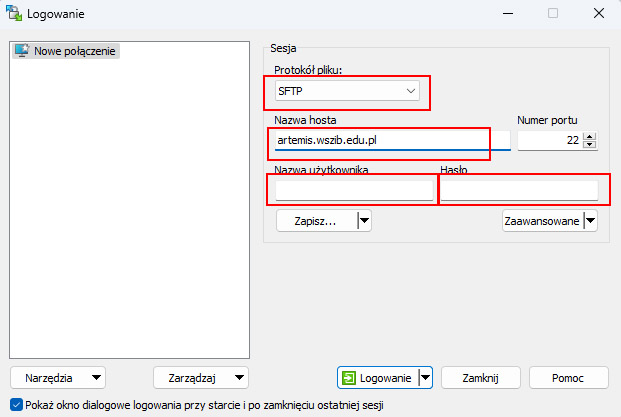
\includegraphics[scale=0.45]
    {./Presentations-pictures/Miscancellous-pictures/Artemis.jpg}


    \caption{Logowanie~się do systemu Artemis za pomocą programu
      Win\textsc{scp}.}


    \label{fig:Artemis-system}

  \end{figure}

\end{frame}
% ######################################












% ################################################
\section{Włączanie powłoki BASH}
% ################################################


% ######################################
\begin{frame}
  \frametitle{Powłoka BASH}

  \vspace{-0.5em}


  \begin{figure}

    \centering


    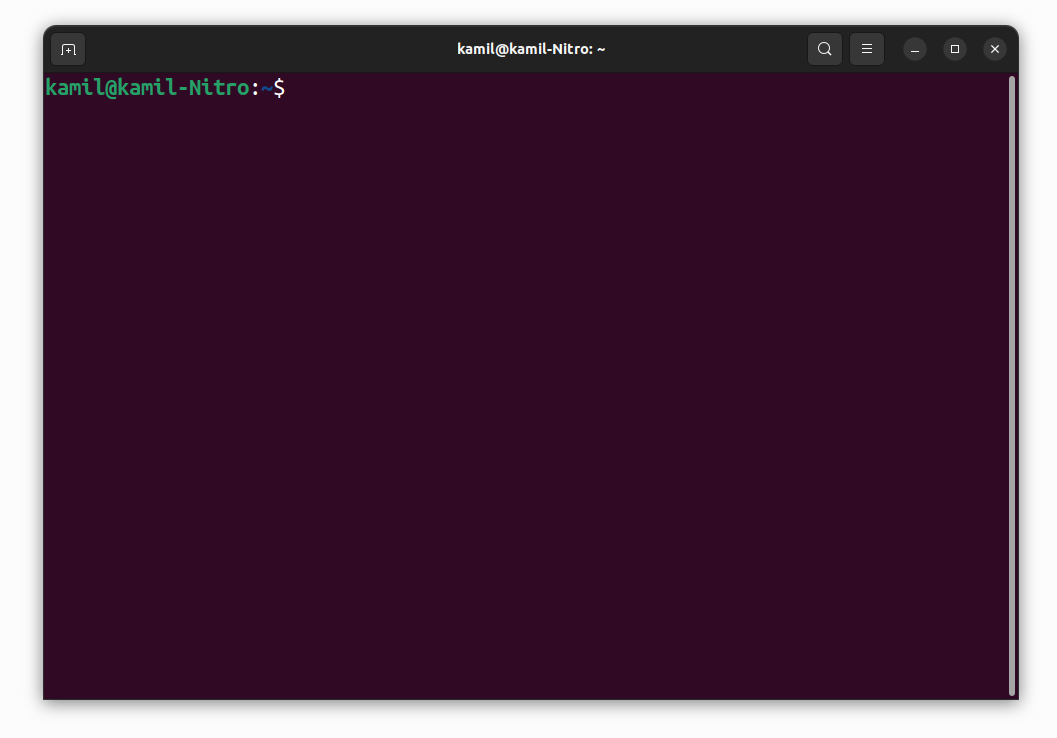
\includegraphics[scale=0.23]
    {./Presentations-pictures/Miscancellous-pictures/BASH-shell.png}


    \caption{Przykładowy wygląd włączonej powłoki \textsc{bash}, naszego
      głównego narzędzia pracy na tym przedmiocie.}


    \label{fig:BASH-shell}

  \end{figure}

\end{frame}
% ######################################





% ######################################
\begin{frame}
  \frametitle{Postęp technologiczny}

  \vspace{-0.5em}


  \begin{figure}

    \label{fig:Evolution-of-OS}

    \centering


    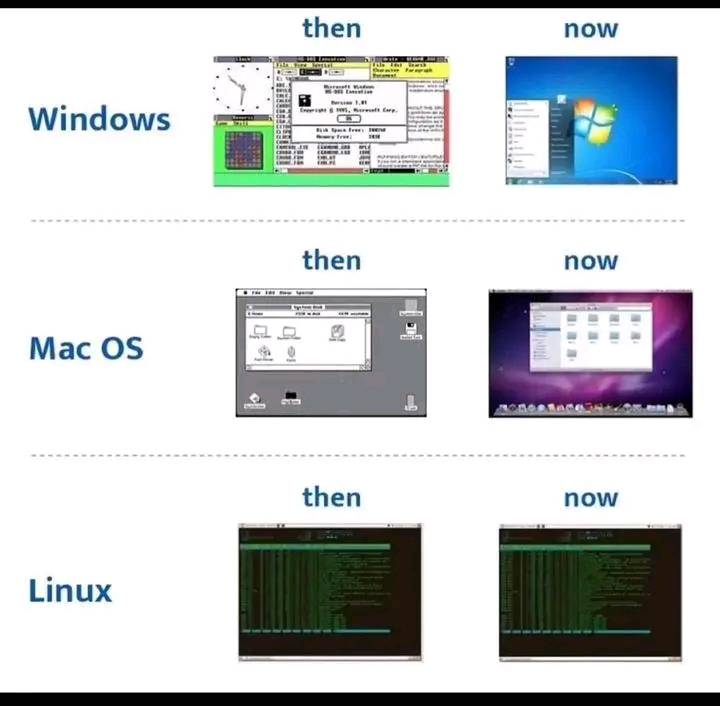
\includegraphics[scale=0.3]
    {./Presentations-pictures/Miscancellous-pictures/Evolution-of-operating-systems.jpg}

  \end{figure}

\end{frame}
% ######################################





% ######################################
\begin{frame}
  \frametitle{Włączanie powłoki}


  \textit{Gdy samochody rozwijały~się tak jak komputery, to dziś
    Rolls-Royce kosztowałby jakieś 100\$, przejeżdżałaby milion mil na
    jednym galonie benzyny i~raz do roku eksplodował, zabijając wszystkich
    w~środku.} \\
  Robert Cringely, \textit{InfoWorld}, tłum. swobodne. Por.~str.~221
  \parencite{Garfinkel-Weise-Strassmann-The-UNIX-HATERS-Handbook-Pub-1994}.

  Naszym główny narzędziem na tych zajęciach będzie powłoka
  (ang. \textit{shell}) \textsc{bash}, więc upewnijmy~się, że~umiemy ją
  włączyć, co na samy początku może być naprawdę niewdzięcznym zadaniem.
  W~pierwszym kroku proszę wcisnąć \texttt{Ctrl-Alt-t} i~zobaczyć, czy~się
  otworzy.

  Jeśli to nie zadziała, to proszę pochodzić kursorem po ekranie,
  aż~znajdziemy okienko „Szukaj”, „Wyszukaj” lub jeszcze jakaś inna nazwa.
  Proszę tam wpisać „Terminal”, „Konsola” lub „Consol” i~zobaczyć, czy
  wyświetli~się odpowiednia ikona do kliknięcia.

  % !!!!!!! Nie usuwać.
  % Istnieje wiele wartych uwagi materiałów do nauki \textsc{bash}a, niekiedy
  % dość już wiekowych. Przykładowo, można sięgnąć do tutorialu
  % Gilesa Orra
  % \colorhref{https://www.gilesorr.com/bashprompt/howto/}
  % {\textit{Bash Prompt HOWTO}} \parencite{Orr-Bash-Prompt-HOWTO-Ver-2009}.

\end{frame}
% ######################################










% ##################
\begin{frame}
  \frametitle{Z~BASHem dzieje~się coś dziwnego}


  Błędne wprowadzenie jakiegoś polecenia może spowodować, że~\textsc{bash}
  przestanie reagować, lub będzie reagował zupełnie nie tak jak tego
  oczekujemy. Ponieważ \textsc{bash} nie wiem czym jest litość, w~zależności
  od tego co konkretnie~się zepsuło, dokładna procedura naprawy jest inna.

  Jednak w~większości przypadków, by wrócić do normalnej pracy wystarczy
  wcisnąć \alert{raz} \texttt{Ctrl-d}. Należy zaznaczyć, że~wciśnięcie
  \texttt{Ctrl-d} \alert{więcej niż raz} może spowodować zamknięcie powłoki
  \textsc{bash} i~potrzeby zrobienia kilku rzeczy ponownie. Z~tego też
  powodu, początkujący \alert{nigdy} nie powinni używać tego skrótu, jeśli
  wszystko działa jak trzeba.

  Mimo tych zastrzeżeń, \texttt{Ctrl-d} jest jednym z~naszych najlepszych
  przyjaciół.

\end{frame}
% ##################










% ######################################
\section{Podstawy pracy z~poziomu powłoki BASH}
% ######################################



% ##################
\begin{frame}
  \frametitle{Kilka słów wstępnych i~ostrzeżeń}


  Przed chwilą mówiliśmy, że~\textsc{bash} nie zna słowa litość i~każda
  drobna zmiana może wszystko zniszczyć. Jednocześnie nasza swoboda nie jest
  całkiem zerowa (choć może często sprawiać takie wrażenie), więc
  podając tutaj różne polecenia, musimy zdecydować~się na pewno konwencje.
  Proszę więc mieć świadomość, że~\alert{pewne} zmiany można wprowadzić
  do~poleceń i~nie zmienią one sposób ich działania.

  Jednak zasady które mówią co \alert{można} zmienić w~poleceniu
  \textsc{bash}a, bez obrócenia wszystkiego w~ruiny, są często nieintuicyjne
  i~skomplikowane. Ponieważ zaś zawsze $1000$ różnych rzeczy może zepsuć
  dane polecenie, zdecydowaliśmy, że~w~tym kursie będziemy starali~się
  podawać te wersje poleceń, które my uważamy za~optymalne i~które działają
  poprawnie, nie zaś wnikać w~pokrętne zasady „możesz zmienić to tak i~tak,
  ale~już nie w~ten sposób”.

\end{frame}
% ##################





% ##################
\begin{frame}
  \frametitle{Kilka słów wstępnych i~ostrzeżeń}


  Testowanie różnych wariantów tych poleceń, sprawdzanie który ich wariant
  działa, a~który nie, jest oczywiście czymś dobrym, co pozwala lepiej
  zrozumieć powłokę \textsc{bash}, więc bardzo nasz cieszy, gdy ktoś tego
  próbuje. Zajmuje to jednak czas, a~większość ludzi pragnie by „komputer
  zrobił to co trzeba”, nie zaś zgłębiać wszystkie niuanse jego pracy.
  Biorąc to wszystko pod uwagę, uznaliśmy, że~obecne sposób wykładu jest
  dobrym wyborem.

  Wszystko utrudnia dodatkowy fakt, że~od czasu do czasu można~się natknąć
  na~dwa warianty poleceń \textsc{bash}a, które działają tak samo, tylko,
  że~to nie do końca prawda. Działają tak samo w~$90\%$ przypadków,
  w~pozostały~$10\%$, działają inaczej. By uniknąć niekończących~się
  dywagacji na temat dzielenia włosa na czworo w~\textsc{bash}u, proszę
  przyjąć, że~jeśli polecenie nie działa jak trzeba, należy~się upewnić,
  iż~są one \alert{dokładnie} takie jak podano tutaj.

\end{frame}
% ##################





% ##################
\begin{frame}
  \frametitle{Kilka słów wstępnych i~ostrzeżeń}


  Do problemu, której wersji poleceń/kodu \textsc{bash}a należy używać,
  wrócimy jeszcze przy okazji pisania skryptów dla tej powłoki. To jednak
  na tą chwilę dość odległy temat.

  Pomimo tego, że~staramy~się dokładnie przetestować wszystkie podane
  w~tych wykładach polecenia \textsc{bash}a, nie możemy wykluczyć tego,
  że~popełnimy jakiś błąd. Dlatego bardzo prosimy by każdy, kto taki
  znajdzie, przesłał go nam pod adres \email.

\end{frame}
% ##################





% ##################
\begin{frame}
  \frametitle{Zaczynamy}


  Zacznijmy od przyjęcia, że~pracujemy na komputerze jako użytkownik,
  którego nazwa w~systemie operacyjnym została wybrana jako \texttt{adam}.
  Jeśli włączymy konsolę zobaczymy pewnie coś takiego: \\
  \texttt{adam:$\sim$\$} \\
  Od tego momentu będziemy zwykle skracali ten znak zachęty \\
  (ang.~\textit{prompt}) do symbolu \texttt{\$}. Przepisywanie pełnej jego
  postaci wnosi bardzo mało informacji, za~to zabiera sporo miejsca.

  Na początku zajmiemy~się tym, jak poruszać~się po systemie plików
  i~katalogów. Na pewno wiedzą Państwo, że~na komputerze znajdują~się
  katalogi (ang.~\textit{directories}), zwane też folderami, które zawierają
  pliki i~inne katalogi. Z~punktu widzenia systemu GNU/Linux
  katalog jest plikiem, jedynie specjalnego rodzaju. Dla tego systemu
  wszystko jest plikiem lub procesem.

\end{frame}
% ##################





% ######################################
\begin{frame}
  \frametitle{Polecenia}


  \textit{Powłoka systemowa (ang.)} shell \textit{jest programem służącym
    do~uruchamiania innych programów. Umożliwia ona użytkownikom wydawanie
    poleceń i~stanowi podstawowy interfejs między nimi a~systemem
    operacyjnym. Gdy loguję~się do systemu Unix, moja klawiatura jest
    podłączona do działającej instancji (kopii) powłoki systemowej.
    Mogę napisać polecenia~-- zwykle pojedynczo~-- a~powłoka uruchamia
    je po kolei; po zakończeniu każdego z~nich jest gotowa do~następnego.
    Sesja może więc wyglądać tak jak poniżej, przy czym \$ jest
    wyświetlanym przez powłokę znakiem zachęty, dzięki któremu wiem,
    że~oczekuje ona na moje działania.} \\[0.3em]
  Str.~$88$, \parencite{Kernighan-Jak-Unix-tworzyl-historie-Pub-2021}.

\end{frame}
% ######################################





% ##################
\begin{frame}
  \frametitle{Polecenia}


  Podstawy działania katalogów w~systemie GNU/Linux są w~zasadzie takie
  same jak w~systemie Windows, musimy~się jedynie przyzwyczaić do innych
  konwencji używanych w~tym systemie. Dużo większym wyzwaniem zapewne
  będzie zamienienie środowiska graficznego (\textsc{gui},
  ang.~\textit{Graphic User Interface}) na pracę z~poziomu powłoki.

  Podstawą pracy w~powłoce \textsc{bash} jest korzystanie z~poleceń (ang.
  \textit{commands}). Bez wnikania w~szczegóły, każde polecenie posiada
  nazwę i~wykonuje pewne działanie. By wykonać dane polecenie w~powłoce
  należy najpierw wpisać jej nazwę, następnie zaś jej odpowiednie
  opcje (flagi) i~argumenty. Część poleceń można wykonać bez wpisywania
  opcji czy~argumentów.

  Trzeba~się niestety przyzwyczaić do tego, że~nazwy poleceń, jak i~nazwy
  ich opcji tych poleceń w~systemie GNU/Linux potrafią być dość dziwne
  i~trudne do~zapamiętania.

\end{frame}
% ##################





% ##################
\begin{frame}
  \frametitle{Polecenia}


  Podstawowych poleceń systemu GNU/Linux jest około~$100$, do tego każde ma
  kilkanaście albo więcej opcji. Z~tego powodu nauka ich jest bardzo
  czasochłonna i~niełatwa. Teoretycznie w~każdej chwili w~\textsc{bash}u
  możemy skorzystać z~manuala (podręcznika), gdzie są opisy wszystkich
  poleceń. W~praktyce, żeby zrozumieć jego treść, wymagana jest już dość
  spora wiedza.

  Zdecydowaliśmy~się przyjąć następujące podejście. Naszym głównym celem
  jest przekazanie Państwu umiejętności pracy spod powłoki \textsc{bash}
  w~możliwie krótki i~bezbolesny sposób. Dlatego też, dość szybko
  wprowadzimy możliwie dużo poleceń, bez zagłębiania~się w~zbyt wiele
  szczegółów. Niekiedy będziemy wracać do wcześniej już omówionych poleceń,
  by uzupełnić wiadomości o~nich. Wyczerpujące omówienie wszystkich
  podstawowych poleceń i~tak zabrałoby zbyt dużo czasu, to zaś podejście
  uważamy, za rozsądny kompromis.

\end{frame}
% ##################





% ##################
\begin{frame}
  \frametitle{Polecenie \texttt{ls}}


  Zacznijmy od~polecenia
  \colorhref{https://linux.fandom.com/pl/wiki/Ls}{\texttt{ls}}. Jego nazwa
  pochodzi prawdopodobnie od~ang.~\textit{List fileS}, ale są różne opinie
  na ten temat. Polecenie to wyświetla zawartość katalogu w~którym~się
  znajdujemy, z~tego powodu wynik działania tego polecenia będzie~się cały
  czas zmieniać, jednym z~możliwych może być ten przedstawiony poniżej. \\
  \texttt{\$ ls} \\
  \texttt{{\color{jAxisBlue} Dokumenty}} \quad
  \texttt{introduction-to-GNU-linux.pdf} \quad
  \texttt{{\color{jAxisBlue} Pobrane}}

  Polecenie \texttt{ls} jest przykładem takiego polecenia, które można
  uruchomić bez dodatkowych opcji czy argumentów, ono samo ustali w~jakim
  katalogu jesteśmy i~wypisze jego zawartość.

  Obecnie jest standardem, że~powłoka używa kolorów i~różnych typów fontów,
  by~informować nas o~typie i~własnościach pliku. W~przykładzie powyżej
  nazwy katalogów są wyróżnione na niebiesko, trzeba jednak pamiętać,
  że~wszystko to~zależy od~konkretnych ustawień systemu operacyjnego
  i~łatwo może zostać zmienione.

\end{frame}
% ##################





% ##################
\begin{frame}
  \frametitle{Polecenie \texttt{pwd}}


  Kolejnym poleceniem jest
  \colorhref{https://www.arturpyszczuk.pl/commands-pwd.html}{\texttt{pwd}}
  od ang.~\textit{Print Working Directory}, rezultat jego działania można
  zobaczyć poniżej. \\
  \texttt{\$ pwd} \\
  \texttt{/home/adam}

  Ta krótka linia zawiera bardzo dużo informacji i~potrzebujemy przynajmniej
  kilka z~nich wyjaśnić. Sposób w~jaki pliki i~katalogi są ułożone na~dysku
  jest zdefiniowane przez \textbf{system plików} danego systemu
  operacyjnego i~ten używany w~systemie GNU/Linux różni~się mocno tego
  w~systemie Windows.

  Zacznijmy od kilku uwag odnośnie notacji. Jeśli pracowalibyśmy w~tym
  ostatnim systemie i~na dysku~C znajdowałby~się
  katalog \texttt{Systemy-operacyjne-Ćwiczenia} a~w~nim katalog
  \texttt{Zajęcia-01}, to ścieżka do niego miałaby postać: \\
  \texttt{C:\textbackslash\textbackslash
    Systemy-operacyjne-Ćwiczenia\textbackslash Zajęcia-01} \\

\end{frame}
% ##################





% ##################
\begin{frame}
  \frametitle{System plików}


  Odpowiednikiem ścieżki z~systemu Windows: \\
  \texttt{C:\textbackslash\textbackslash
    Systemy-operacyjne-Ćwiczenia\textbackslash Zajęcia-01} \\
  w~systemie GNU/Linux byłaby ścieżka: \\
  \texttt{/home/adam/Systemy-operacyjne-Ćwiczenia/Zajęcia-01} \\
  Widzimy więc, że~gdy Windows do oddzielania nazw katalogów i~plików
  używa symbolu „backslasha”: „\texttt{\textbackslash}”, to GNU/Linux
  używa symbolu „slasha”: „\texttt{/}”. Jest to stosunkowo mała różnica,
  ale trzeba~się do niej przyzwyczaić.

  Poważniejsza różnica jest następująca. Komputery z~systemem GNU/Linux
  mogą posiadać wiele dysków, nie jest to żadnym problemem, ale~system
  plików GNU/Linuxa nie zna pojęcia dysku jako takiego. W~systemie GNU/Linux
  istnienie naczelny katalog zwany rootem, czyli po polsku „korzeniem”,
  w~którym zawierając~się wszystkie inne pliki oraz katalogi, nieważne na
  którym fizycznym dysku są one umieszczone. Katalog root oznaczamy
  symbolem~„\texttt{/}”.

\end{frame}
% ##################





% % ##################
% \begin{frame}
%   \frametitle{System plików}


%   Odpowiednikiem ścieżki z~systemu Windows: \\
%   \texttt{C:\textbackslash\textbackslash
%     Systemy-operacyjne-Ćwiczenia\textbackslash Zajęcia-01} \\
%   w~systemie GNU/Linux byłaby ścieżka: \\
%   \texttt{/home/adam/Systemy-operacyjne-Ćwiczenia/Zajęcia-01} \\
%   Widzimy więc, że~gdy Windows do oddzielania nazw katalogów i~plików
%   używa symbolu „backslasha”: „\texttt{\textbackslash}”, to GNU/Linux
%   używa symbolu „slasha”: „\texttt{/}”. Jest to stosunkowo mała różnica,
%   ale trzeba~się do niej przyzwyczaić.

%   Poważniejsza różnica jest następująca. Komputery z~systemem GNU/Linux
%   mogą posiadać wiele dysków, nie jest to żadnym problemem, ale~system
%   plików GNU/Linuxa nie zna pojęcia dysku jako takiego. W~systemie GNU/Linux
%   istnienie naczelny katalog zwany rootem, czyli po polsku „korzeniem”,
%   w~którym zawierając~się wszystkie inne pliki oraz katalogi, nieważne na
%   którym fizycznym dysku są one umieszczone. Katalog root oznaczamy
%   symbolem~„\texttt{/}”.

% \end{frame}
% % ##################





% ##################
\begin{frame}
  \frametitle{System plików}


  Wróćmy do polecenia \\
  \texttt{\$ pwd} \\
  \texttt{/home/adam} \\
  Linię \texttt{/home/adam} czytamy „W~katalogu root („\texttt{/}”)
  znajduje~się katalog \texttt{home}, w~nim zaś znajduje~się katalog
  \texttt{adam}.” Polecenie \texttt{pwd} podaje więc w~którym katalogu~się
  obecnie znajdujemy, za~pomocą ścieżki, która zaczyna~się od katalogu root:
  „\texttt{/}”.

  Katalog w~którym obecnie jesteśmy nosi nazwę \textbf{katalogu roboczego}
  (ang.~\textit{working directory}), a~jak powiedzieliśmy \texttt{pwd} jest
  akronimem od~\textit{Print Working Directory}, czyli „wyświetl katalog
  roboczy”.

  Ścieżkę podającą lokalizację katalogu lub pliku nazywamy
  \textbf{ścieżką bezwzględną}, jeśli zaczyna~się ona od katalogu root.
  W~przeciwnym razie mówimy o~\textbf{ścieżce względnej} (podawanej
  względem innego katalogu niż root).

\end{frame}
% ##################





% ##################
\begin{frame}
  \frametitle{System plików}


  Bez wielkich uproszczeń można przyjąć, że~\textsc{bash}u \alert{każdy}
  ciąg symboli zaczynający od~symbolu „\texttt{/}” zostanie zinterpretowany
  jako ścieżka do jakiegoś pliku lub katalogu. Z~tego powodu trzeba
  \alert{bardzo} uważać przy stosowaniu symbolu~„\texttt{/}”.

  W~szczególności, gdy stosujemy symbol „\texttt{/}”, trzeba zwracać dużą
  uwagę na~spacje. Ścieżka postaci \\
  \texttt{/home/adam} \\
  jest poprawna. Ale już ścieżka \\
  \texttt{/ home/adam} \\
  jest \alert{błędna}! To w~jaki sposób jest błędna, to omówimy innym
  razem. Doświadczenie uczy, że~na początku sprawia to ludziom
  bardzo dużo problemów.

  To, że~główny katalog nosi nazwę „korzenia” (ang.~\textit{root}) nie jest
  przypadkiem, ale do tej kwestii wrócimy innym razem.

\end{frame}
% ##################





% ##################
\begin{frame}
  \frametitle{Katalog domowy}


  W~systemie GNU/Linux każdy użytkownik ma swój katalog domowy, w~którym
  może przechowywać potrzebne mu pliki. Standardowo, choć mogą być wyjątki,
  użytkownik \texttt{adam} otrzyma katalog \texttt{/home/adam}, użytkownik
  \texttt{barbara} katalog \texttt{/home/barbara},~etc. Katalog domowy
  bieżącego użytkownika posiada też alternatywną nazwę „$\sim$”. Stąd znak
  zachęty \\
  \texttt{adam:$\sim$\$} \\
  przekazuje nam informację, że~działamy jako użytkownik \texttt{adam}
  i~znajdujemy~się w~jego katalogu domowym.

  Załóżmy, że~katalogu domowym znajduje~się katalog o~nazwie
  \texttt{Systemy-operacyjne-Ćwiczenia}. By sprawdzić, czy tak jest
  naprawdę możemy użyć polecenia \texttt{ls}: \\
  \texttt{\$ ls} \\
  \texttt{{\color{jAxisBlue} Dokumenty}} \quad
  \texttt{introduction-to-GNU-linux.pdf} \quad
  \texttt{{\color{jAxisBlue} Pobrane}} \\
  \texttt{{\color{jAxisBlue} Systemy-operacyjne-Ćwiczenia}} \\

\end{frame}
% ##################





% ##################
\begin{frame}
  \frametitle{Polecenie \texttt{cd}}


  Jeśli w~bieżącym katalogu znajduje~się katalog
  \texttt{Systemy-operacyjne-Ćwiczenia} to możemy do niego wejść
  używając polecenia
  \colorhref{https://linux.fandom.com/pl/wiki/Cd}{\texttt{cd}}
  (od ang.~\textit{Change Directory}): \\
  \texttt{adam:$\sim$\$ cd Systemy-operacyjne-Ćwiczenia} \\
  \texttt{adam:$\sim$/Systemy-operacyjne-Ćwiczenia\$} \\
  Wyjątkowo zapisaliśmy pełniejszą wersję znaku zachęty, by podkreślić,
  iż~informuje on~nas w~którym katalogu jesteśmy. Mianowicie ścieżka
  \texttt{$\sim$/Systemy-operacyjne-Ćwiczenia} informuje nas, że~w~katalogu
  domowych użytkownika \texttt{adam} znajduje~się katalog
  \texttt{Systemy-operacyjne-Ćwiczenia} i~w~nim właśnie jesteśmy.

  Użyte wyżej polecenie \texttt{cd} jest przykładem polecenia, które
  pobiera argument, mianowicie nazwę katalogu do którego możemy wejść.
  W~istocie polecenie to pozwala nam na bardzo swobodne poruszanie~się
  po systemie plików, jeśli opanujemy dobrze zapis ścieżek w~GNU/Linuxie,
  ale wszystko po kolei.

\end{frame}
% ##################





% ##################
\begin{frame}
  \frametitle{Polecenie \texttt{cd}}


  Załóżmy, że~teraz chcielibyśmy przejść do katalogu nad nami. By to zrobić
  należy przekazać poleceniu \texttt{cd} argument „\texttt{..}”: \\
  \texttt{adam:$\sim$/Systemy-operacyjne-Ćwiczenia\$ cd ..} \\
  \texttt{adam:$\sim$\$} \\
  Dlaczego jako argument przesyłamy akurat „\texttt{..}” wyjaśnimy w~swoim
  czasie, na razie przyjmijmy, iż~tak po prostu jest. Dla lepszej
  ilustracji tego co~zrobiliśmy, ponownie wypisaliśmy znak zachęty,

  Załóżmy, że~chcemy teraz wejść do katalogu
  \texttt{Systemy-operacyjne-Ćwiczenia} i~utworzyć tam plik
  \texttt{Notatki-z-zajęć.txt}. By utworzyć ten plik możemy skorzystać
  z~polecenia
  \colorhref{https://linux.fandom.com/pl/wiki/Touch}{\texttt{touch}}. Pełna
  sekwencja poleceń będzie wyglądać tak. \\
  \texttt{\$ cd Systemy-operacyjne-Ćwiczenia} \\
  \texttt{\$ touch Notatki-z-zajęć.txt} \\

\end{frame}
% ##################





% ##################
\begin{frame}
  \frametitle{Edycja plików z~pomocą programu gedit}


  Możemy teraz użyć polecenia \texttt{ls} by~się przekonać, czy~plik
  \texttt{Notatki-z-zajęć.txt} został poprawnie utworzony.
  Z~komputerami nigdy nic nie wiadomo, więc warto to sprawdzić.

  W~następnym kroku otworzymy go do edycji za~pomocą programu
  \colorhref{https://gedit-text-editor.org/}{gedit}. By to zrobić
  wpisujemy w~powłoce \\
  \texttt{\$ gedit Notatki-z-zajęć.txt \&} \\
  Proszę pamiętać o~dodaniu na końcu polecenia znaku
  \alert{ampersand}:~„\&”. Inaczej gedit zablokuje nam możliwość wpisywania
  kolejnych poleceń do powłoki i~by ją odzyskać, będziemy musieli
  wyłączyć gedita albo użyć kombinacji poleceń \texttt{jobs} i~\texttt{bg}.

  Czemu uruchomienie gedita bez symbolu ampersanda ma takie skutki, omówimy
  gdy będziemy dyskutowali zagadnienie procesów i~tego jak działają
  w~systemie GNU/Linux. Nie jest to najprostszy temat na świecie.

\end{frame}
% ##################





% ##################
\begin{frame}
  \frametitle{Okienko gedita}


  Jeśli wszystko poszło dobrze, to na ekranie zobaczymy okienko Gedita,
  które wygląda mniej więcej tak jak to na~zdjęciu~\eqref{fig:Gedit-window}.





  \begin{figure}

    \centering

    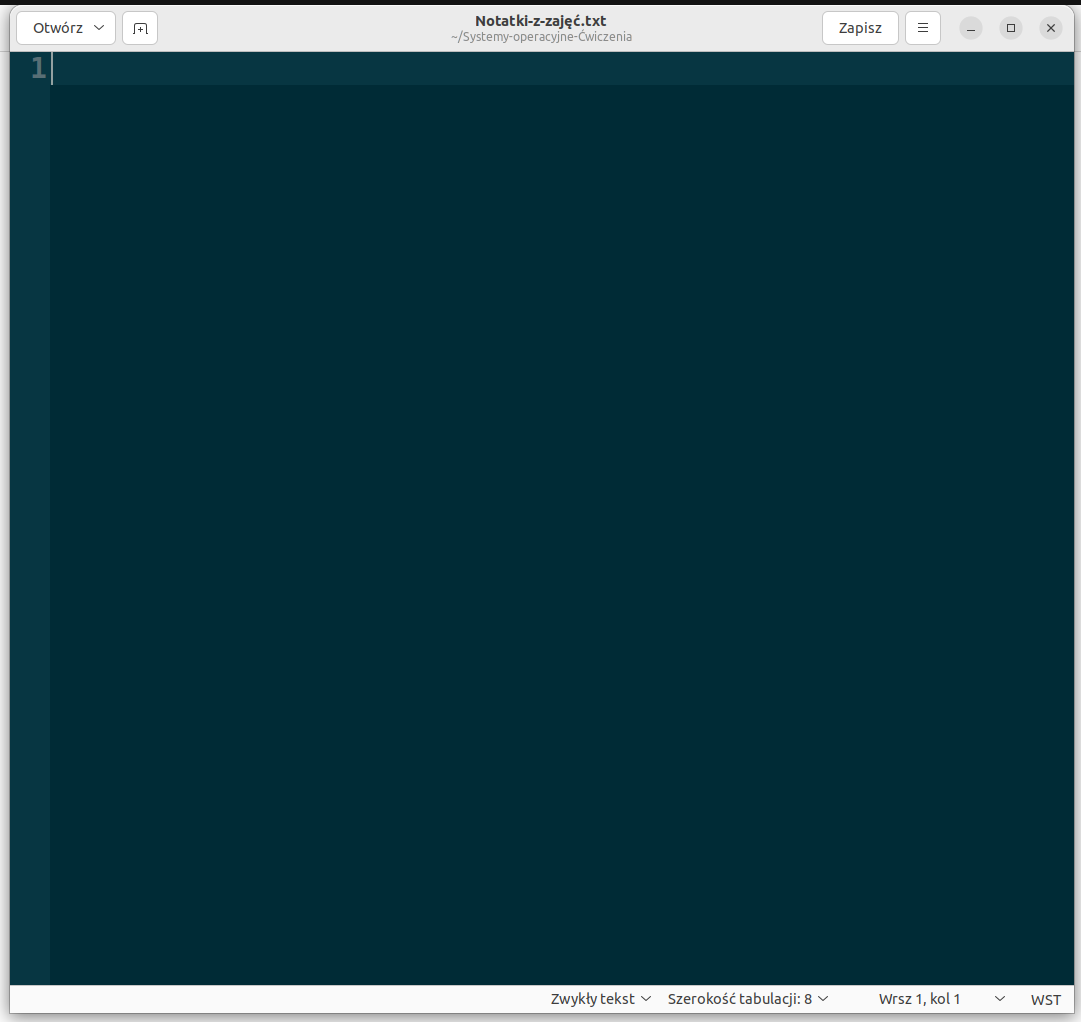
\includegraphics[scale=0.145]
    {./Presentations-pictures/Miscancellous-pictures/gedit-window.png}

    \caption{Otwarte okienko programu gedit.}


    \label{fig:Gedit-window}

  \end{figure}

\end{frame}
% ##################





% ##################
\begin{frame}
  \frametitle{Edytory tekstów}


  Teraz możemy do pliku \texttt{Notatki-z-zajęć.txt} wpisać tekst, choćby
  \textit{Notatki z~przedmiotu „Systemy operacyjne”}. Proszę pamiętać, by
  zapisywać wprowadzone zmiany, służy do tego choćby skrót~\texttt{Ctrl-s}.

  Kilka słów dlaczego wybraliśmy do~edycji plików program gedit. Na~tym
  kursie korzystamy głównie z~niego, gdyż jest on prosty w~obsłudze
  i~w~kilka sekund po jego otwarciu użytkownik może już pisać odpowiedni
  tekst. Zostawiamy jednak Państwu pełną swobodę w~wyborze edytora tekstu.
  Nie jest ważne jakiego programu~się używa, ważne jest, żeby udało~się
  wykonać zadanie jakie przed nami stoi.

  Jeśli chodzi o~edytory dostępne pod systemem GNU/Linux, to w~naszej
  ocenie warto zwrócić uwagę choćby na~dwa owiane już legendą programy
  do edycji tekstu \colorhref{https://www.vim.org/}{vim}
  i~\colorhref{https://www.gnu.org/software/emacs/}{GNU Emacs}.

\end{frame}
% ##################










% ################################################
\section{Czy tylko mi~się wydaje, że~ten system jest dziwny?}
% ################################################


% ######################################
\begin{frame}
  \frametitle{Czy tylko mi~się wydaje, że~ten system jest dziwny?}


  Niejedna z~poznanych przez nas cech systemu operacyjnego, może
  wydawać~się nam dziwna. Czy życie nie mogłoby być prostsze, a~system
  operacyjny bardziej zrozumiały? Odpowiedź na oba pytania brzmi
  „Prawdopodobnie tak”. Dlaczego więc tak nie jest?

  Warto sobie uświadomić, że~niektórzy jeżdżą jeszcze zabytkowymi
  samochodami wyprodukowanymi w~latach $60$-tych XX~wieku. Prawdopodobnie
  gdzieś na świecie działają jakieś komputery wyprodukowane w~tych latach,
  ale większa jest szansa zobaczenia go w~muzeum, niż wykonującego jakąś
  pracę. W~przeciwieństwie do tego, pomysł z~lat $60$-tych mają~się
  świetnie, również w~informatyce. Pracując z~systemami często
  napotykamy~się na jakiś jego fragment, który wymyślono w~owym czasie,
  odbija on więc ówczesny stan wiedzy i~możliwości techniczne. By więc
  zrozumieć pewne osobliwości systemów operacyjnych warto udać~się w~krótką
  podróż w~przeszłość.

\end{frame}
% ######################################





% ######################################
\begin{frame}
  \frametitle{Trochę historii}


  Główne przesłanie tej historii jest następujące. Systemy operacyjne
  których dziś używamy, wyewoluowały do swojej obecnej formy formy
  na przestrzeni dekad, wchłaniając i~łącząc pomysły pochodzące
  z~różnorakich źródeł. Stąd ich dzisiejszy czas może sprawiać wrażenie
  przestarzałego, bałaganiarskiego i~pełnego niekonsekwencji. Jest to prawdą
  w~przypadku w~zasadzie wszystkich popularnych systemów operacyjnych, nie
  tylko omawianego przez nas GNU/Linuxa.

  Zaczynamy w~późnej epoce brązu komputerów, czyli roku~$1965$.
  W~owym roku w~USA, uczelnia M.I.T oraz firmy General Electrics i~Bell
  Labs zaczynają pracę nad systemem operacyjnym
  \colorhref{https://en.wikipedia.org/wiki/Multics}{\textsc{multics}}
  (ang.~\textit{MULTiplexed Information and Computing Service}). Prace
  nas systemem \textsc{multics} okazały~się wyjątkowo skomplikowane i~sam
  projekt odniósł jedynie częściowy sukces. Z~uwagi na trudności
  przy tworzeniu tego systemu Bell Labs wycofały~się z~projektu
  w~roku $1969$.

\end{frame}
% ######################################





% ######################################
\begin{frame}
  \frametitle{Ken Thompson i~jego współpracownicy}


  Jednym z~ludzi, który pracował z~ramienia Bell Labs nad \textsc{multics}em
  jest \colorhref{https://en.wikipedia.org/wiki/Ken\_Thompson}
  {Ken Thompson}. Po wycofaniu~się Bell Labs z~tego projektu, Thompson
  poszukując nowych problemów do rozwiązania, zaczyna pisać programy na
  znajdujący~się w~Bell Labs i~wówczas już rzadko używany komputer
  \colorhref{https://en.wikipedia.org/wiki/PDP-7}{PDP-$7$}.
  W~trackie pracy nad nimi w~pewnym momencie dochodzi do~wniosku,
  że~niewiele mu brakuje do stworzenia systemu operacyjnego. W~ten sposób
  powstaje system operacyjny \textsc{unix}, którego pierwsza wersja
  jest gotowa na jesień $1969$~roku.

  Sama nazwa „\textsc{unix}”,
  jak zgadzają~się wszyscy biorący udział w~jego tworzeniu, jest
  nawiązaniem, i~to dość złośliwym do nazwy „\textsc{multics}”.
  Związane jest to z~powszechną krytyką, że~\textsc{multics} próbował
  osiągnąć zbyt wiele rzeczy na raz i~to nie wyszło mu na zdrowie,
  a~nowy system będzie skupiał~się na robieniu kilku rzeczy dobrze. Stąd
  „multi” zmieniono na „unit” i~powstała nazwa \textsc{unix}, por.
  str.~???.

\end{frame}
% ######################################





% ######################################
\begin{frame}
  \frametitle{Ken Thompson i~jego współpracownicy}


  Do Thompsona w~pracy nad \textsc{unix}em dołącza wielu wybitnych
  informatyków, pracujących wtedy w~Bell Labs, jak ???

  System \textsc{unix} jest pierwszym bezpośrednim przodkiem używanego
  przez nas systemu GNU/Linux, jednak droga od jednego do~drugiego
  jest dość długa i~wyboista.

\end{frame}
% ######################################





% ######################################
\begin{frame}
  \frametitle{Ken Thompson i~jego współpracownicy}



  \begin{figure}

    \centering


    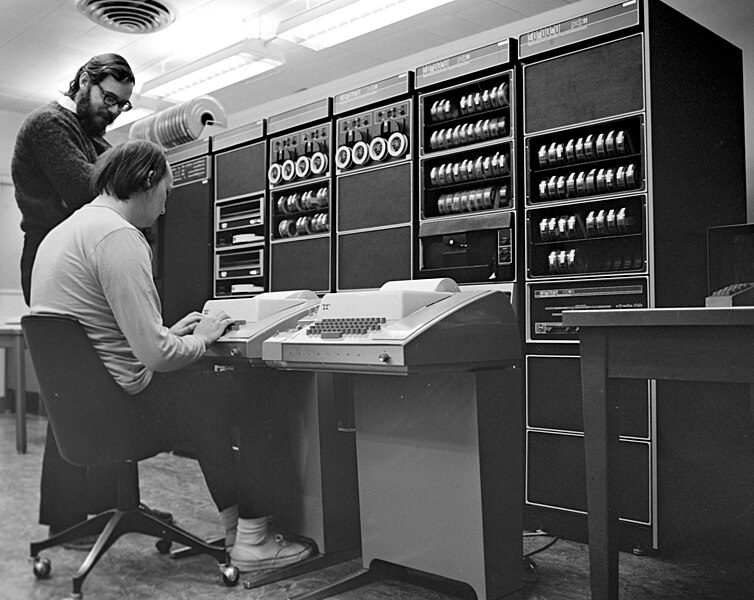
\includegraphics[scale=0.3]
    {./Presentations-pictures/OS-heroes-Pictures/Dennis-Ritchie-Ken-Thompson-around-year-1972.jpg}


    \caption{Ken Thompson (siedzi) i~Dennis Ritchie przy komputerze
      typu PDP-$11$, około roku $1972$-ego.}


    \label{fig:Ritchie-Thompson-around-year-1972}

  \end{figure}

\end{frame}
% ######################################





% ######################################
\begin{frame}
  \frametitle{Ken Thompson i~jego współpracownicy}


  Zdjęcie \eqref{fig:Ritchie-Thompson-around-year-1972} przedstawia Kena
  Thompsona i~Denisa Ritchiego pracujących na komputerze typu
  \colorhref{https://en.wikipedia.org/wiki/PDP-11}{PDP-$11$}, za~pomocą
  dalekopisu
  \colorhref{https://en.wikipedia.org/wiki/Teletype\_Model\_33}
  {Model~$33$ Teletype}. Współtwórca \textsc{unix}a Brian
  W.~Kernighan opatrzył to zdjęcie takim komentarzem.

  \textit{Rysunek 3.1 [u~nas \eqref{fig:Ritchie-Thompson-around-year-1972}]
    przedstawia zrobione na~potrzeby} public relations \textit{w~$1972$
    zdjęcie Kena Thompsona i~Dennisa Ritchiego pracujących nad PDP-$11$
    wyposażona we wczesną wersję Uniksa. Sam komputer najprawdopodobniej
    był specyficznym wariantem PDP-$11$ o~nazwie PDP-$11/20$. Niewielkie,
    okrągłe obiekty znajdujące~się mniej więcej na wysokości głowy, to
    DECtapes~-- napędy z~taśmą magnetyczną, które umożliwiały przechowywanie
    $144\text{K}$ słów $18$-bitowych [$324$ kilobajty pamięci]. Ponieważ
    pozwalały one na odczyt i~zapis pojedynczych bloków, mogły służyć jako
    tymczasowe, wolne, ale niezawodne dyski; taśmy były wymienne, używano
    ich więc też do~archiwizacji danych.}
  Str.~$64$, \parencite{Kernighan-Jak-Unix-tworzyl-historie-Pub-2021}.

\end{frame}
% ######################################





% ######################################
\begin{frame}
  \frametitle{Ken Thompson i~jego współpracownicy}


  \textit{Ken pisze na dalekopisie Model~$33$ Teletype~-- solidnym,
    ale~wolnym i~hałaśliwym urządzeniu, będącym w~istocie sterowaną przez
    komputer elektromechaniczną maszyną do~pisania, która potrafiła pisać
    tylko dużymi literami, w~tempie do~$10$ znaków na sekundę. Model~$33$
    pochodzi z~$1963$ roku, ale wcześniejsze wersje były w~powszechnym
    użyciu już od początku lat~$30$.}

  \textit{Teletype Corporation była częścią AT\&T i~urządzenia Teletypes
    były powszechnie używane w~Bell System i~innych ośrodkach
    do~wysyłania wiadomości; dopiero w~późniejszym czasie zaczęto
    podłączać je do komputerów. To, co zostało wprowadzone na klawiaturze
    Teletype, trafiało do~komputera, a~rezultaty były drukowane (dużymi
    literami) na długiej roli papieru; na~zdjęciu~są widoczne górne
    fragmenty tych rolek. Jak sądzę, jednym z~powodów bardzo krótki
    nazw wielu poleceń Uniksa było to, że~pisanie na Modelu~$33$ wymagało
    niemałej siły, a~drukowanie przebiegało wolno.}
  Str.~$65$, \parencite{Kernighan-Jak-Unix-tworzyl-historie-Pub-2021}.

\end{frame}
% ######################################






% ######################################
\begin{frame}
  \frametitle{Dlaczego?}


  Jak Państwo widzą,

\end{frame}
% ######################################





% ######################################
\begin{frame}
  \frametitle{To tylko część tej historii}


  To co przedstawiliśmy tutaj jest tylko drobnym wycinkiem historii, która
  doprowadziła do powstania używanych przez nas systemów operacyjnych,
  takich jak GNU/Linux.

  Jeśli ktoś chce lepiej poznać tę historię to powinien w~pierwszym rzędzie
  sięgnąć do krótkiej i~bardzo pięknej książki Briana W.~Kernighan
  \textit{Jak Unix tworzył historię}
  \parencite{Kernighan-Jak-Unix-tworzyl-historie-Pub-2021}, która była
  już przez nas wielokrotnie cytowana. Jak sama jej tytuł wskazuje, książka
  ta dotyczy głównie systemu \textsc{unix}, jego powstania i~rozwoju. Jednak
  w~ostatniej części, głównie w~rozdziałach ??? i~??? opisuje drogę, jaka
  wiodła od~\textsc{unix}, do~systemu GNU/Linux. Cała zaś książka jest
  kopalnią informacji na temat, tego kiedy, gdzie i~dlaczego powstały znane
  nam dziś części naszych systemów operacyjnych.

\end{frame}
% ######################################



% % ##################
% \jagiellonianendslide{?????}
% % ##################










% ####################################################################
% ####################################################################
% Bibliography

\printbibliography





% ####################################################################
% End of the document

\end{document}
